\ifx\wholebook\relax\else
\documentclass[twoside]{book}
\usepackage[active]{srcltx}
\usepackage[LY1]{fontenc}
\usepackage{url}
\makeatletter
\def\url@leostyle{%
  \@ifundefined{selectfont}{\def\UrlFont{\sf}}{\def\UrlFont{\sffamily}}}
\makeatother
% Now actually use the newly defined style.
\urlstyle{leo}

\usepackage{graphicx}
\def\etc{{\textit{etc}}}
\def\eg{{\textit{e.g.}}}
\def\ie{{\textit{i.e.}}}
\def\cf{{\textit{c.f.}}\ }
\def\erf{\mathop{\textrm{erf}}}
\def\sign{\mathop{\textrm{sign}}}
\def\prob{\mathop{\textrm{Prob}}}
\def\var{\mathop{\textrm{var}}}
\def\mod{\mathop{\textrm{mod}}}
\def\cor{\mathop{\textrm{cor}}}
\def\cov{\mathop{\textrm{cov}}}
\def\cl{\mathop{\textrm{CL}}}
\def\kg{\mathop{\textrm{Kg}}}
\def\patstyle#1{{\textsc #1}}
\def\th{^{\mathop{\textrm{th}}}}
%\def\st#1{^{\mathop{\rm #1}}}
\def\note#1{\begin{quote}{\textbf{Note:}} #1\end{quote}}
\def\braket#1{\left\langle #1\right\rangle}
\def\order#1{\let\o=#1$\mathcal{O}$\ifx\o 1$\left(n\right)$\else$\left(n^{#1}\right)$\fi}
%\newtheorem{privListing}{Listing}[chapter]
%\newenvironment{listing}{\vskip 3ex\hrule\vskip 1ex\begin{privListing}}{\end{privListing}\hrule\vskip 1ex}
\newtheorem{privExample}{Code example}[chapter]
\newenvironment{codeExample}{\begin{privExample}\begin{quote}\tt}{\end{quote}\end{privExample}}
\def\relboxl#1#2{\hbox to #1\hsize{#2\hfil}}
\def\relboxc#1#2{\hbox to #1\hsize{\hfil #2\hfil}}
\def\relboxr#1#2{\hbox to #1\hsize{\hfil #2}}
\def\transpose#1{\textbf{#1}^{\mathop\textrm{T}}}
\def\inverse#1{\textbf{#1}^{-1}}
%\def\tm{$^{\mathop{\rm TM}}$}
\def\tm{ }
\newenvironment{mainEquation}{\marginpar[\vspace{3 ex} Main
equation$\Rightarrow$]{\vspace{3 ex}$\Leftarrow$Main
equation}\begin{equation}}{\end{equation}}
\def\rubrique#1{\paragraph{#1}\hfil\par\noindent}

\begin{document}
\fi

\chapter{Linear algebra}
\label{ch:linearalgebra}
\begin{flushright}
{\sl On ne trouve pas l'espace, il faut toujours le
construire.}\footnote{Space is not to be found; it must always be
constructed.}\\ Gaston Bachelard
\end{flushright}
\vspace{1 ex} Linear algebra concerns itself with the manipulation
of vectors and matrices. The concepts of linear algebra are not
difficult and linear algebra is usually taught in the first year
of university. Solving systems of linear equations are even taught
in high school. Of course, one must get used to the book keeping
of the indices. The concise notation introduced in linear algebra
for vector and matrix operations allows expressing difficult
problems in a few short equations. This notation can be directly
adapted to object oriented programming.

Figure \ref{fig:linearalgebraclasses} shows the classes described
in this chapter.
\begin{figure}
\centering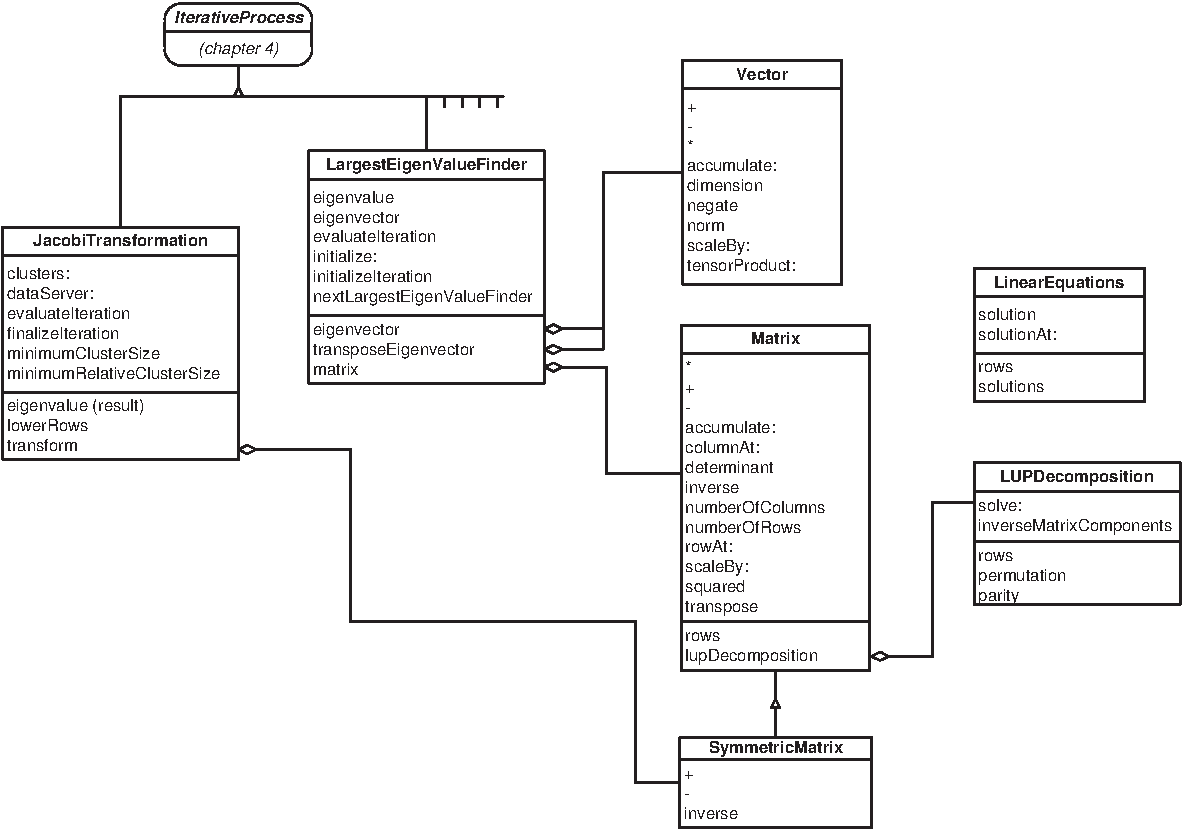
\includegraphics[width=11cm]{Figures/LinearAlgebraClasses}
\caption{Linear algebra classes}\label{fig:linearalgebraclasses}
\end{figure}
Like chapter \ref{ch:function}, this chapter discusses some
fundamental concepts and operations that shall be used throughout
the rest of the book. It might appear austere to many readers
because, unlike the preceding chapters, it does not contains
concrete examples. However, the reader will find example of use of
linear algebra in nearly all remaining chapters of this book.

The chapter begins with a reminder of operations defined on
vectors and matrices. Then, two methods for solving systems of
linear equations are discussed. This leads to the important
concept of matrix inversion. Finally the chapter closes of the
problem of finding eigenvalues and eigenvectors.

\section{Vectors and matrices}
\label{sec:linearalgebra} Linear algebra concerns itself with
vectors in multidimensional spaces and the properties of
operations on these vectors. It is a remarkable fact that such
properties can be studied without explicit specification of the
space dimension\footnote{In fact, most mathematical properties
discussed in this chapter are valid for space with an infinite
number of dimensions (Hilbert spaces).}.

A vector is an object in a multidimensional space. It is
represented by its components measured on a reference system. A
reference system is a series of vectors from which the entire
space can be generated. A commonly used mathematical notation for
a vector is a lower case bold letter, ${\bf v}$ for example. If
the set of vectors ${\bf u}_1,\ldots,{\bf u}_n$ is a reference
system for a space with $n$ dimension, then any vector of the
space can be written as:
\begin{equation}
\label{eq:vectordef}
  {\bf v} = v_1{\bf u}_1+\cdots+v_n{\bf u}_n,
\end{equation}
where $v_1,\ldots,v_n$ are real numbers in the case of a real
space or complex numbers in a complex space. The numbers
$v_1,\ldots v_n$ are called the components of the vector.

A matrix is a linear operator over vectors from one space to
vectors in another space not necessarily of the same dimension.
This means that the application of a matrix on a vector is another
vector. To explain what {\sl linear} means, we must quickly
introduce some notation.

A matrix is commonly represented with an upper case bold letter,
${\bf M}$ for example. The application of the matrix ${\bf M}$ on
the vector ${\bf M}$ is denoted by ${\bf M}\cdot{\bf v}$. The fact
that a matrix is a linear operator means that
\begin{equation}
{\bf M}\cdot\left(\alpha{\bf u}+\beta{\bf v}\right)=\alpha{\bf
M}\cdot{\bf u}+\beta{\bf M}\cdot{\bf v},
\end{equation}
for any matrix ${\bf M}$, any vectors ${\bf u}$ and ${\bf v}$, any
numbers $\alpha$ and $\beta$.

Matrices are usually represented using a table of numbers. In
general, the number of rows and the number of columns are not the
same. A square matrix is a matrix having the same number of rows
and columns. A square matrix maps a vector onto another vector of
the same space.

Vectors and matrices have an infinite number of representations
depending on the choice of reference system. Some properties of
matrices are independent from the reference system. Very often the
reference system is not specified explicitly. For example, the
vector ${\bf v}$ of equation \ref{eq:vectordef} is represented by
the array of numbers $\left( v_1v_2\cdots v_n\right)$ where $n$ is
the dimension of the vector. Writing the components of a vector
within parentheses is customary. Similarly a matrix is represented
with a table of numbers called the components of the matrix; the
table is also enclosed within parentheses. For example, the $n$ by
$m$ matrix ${\bf A}$ is represented by:
\begin{equation}
  {\bf A}=\pmatrix{a_{11}& a_{12}&\ldots& a_{1n}\cr
  a_{21}& a_{22}&\ldots& a_{2n}\cr
  \vdots&\vdots&\ddots&\vdots\cr
  a_{m1}& a_{m2}&\ldots& a_{mn}\cr}.
\end{equation}
The components can be real or complex numbers. In this book we
shall deal only with vectors and matrices having real components.

For simplicity a matrix can also be written with matrix
components. That is, the $n$ by $m$ matrix ${\bf A}$ can be
written in the following form:
\begin{equation}
\label{eq:matrixcomp}
  {\bf A}=\pmatrix{{\bf B}&{\bf C}\cr{\bf D}&{\bf E}\cr},
\end{equation}
where ${\bf B}$, ${\bf C}$, ${\bf D}$ and ${\bf E}$ are all
matrices of lower dimensions. Let ${\bf B}$ be a $p$ by $q$
matrix. Then, ${\bf C}$ is a $p$ by $m-q$ matrix, ${\bf D}$ is a
$n-p$ by $q$ matrix and ${\bf E}$ is a $n-p$ by $m-q$ matrix.

Using this notation one can carry all conventional matrix
operations using formulas similar to those written with the
ordinary number components. There is, however, one notable
exception: the order of the products must be preserved since
matrix multiplication is not commutative. For example, the product
between two matrices expressed as matrix components can be carried
out as:
\begin{equation}
\label{eq:matrixcompmult}
  \pmatrix{{\bf B_1}&{\bf C_1}\cr{\bf D_1}&{\bf E_1}\cr}\cdot
  \pmatrix{{\bf B_2}&{\bf C_2}\cr{\bf D_2}&{\bf E_2}\cr}=
  \pmatrix{{\bf B_1}\cdot{\bf B_2}+{\bf C_1}\cdot{\bf D_2}&
  {\bf B_1}\cdot{\bf C_2}+{\bf C_1}\cdot{\bf E_2}\cr
  {\bf D_1}\cdot{\bf B_2}+{\bf E_1}\cdot{\bf D_2}&
  {\bf D_1}\cdot{\bf C_2}+{\bf E_1}\cdot{\bf E_2}\cr},
\end{equation}
In equation \ref{eq:matrixcompmult} the dimension of the
respective matrix components must permit the corresponding
product. For example the number of rows of the matrices ${\bf
B_1}$ and ${\bf C_1}$ must be equal to the number of columns of
the matrices ${\bf B_2}$ and ${\bf C_2}$ respectively.

Common operations defined on vectors and matrices are summarized
below. In each equation, the left-hand side shows the vector
notation and the right-hand side shows the expression for
coordinates and components.

\vskip 2ex\noindent The sum of two vectors of dimension $n$ is a
vector of dimension $n$:
\begin{equation}
\label{eq:vectorsum}
\begin{tabular}{ccl}
\relboxc{0.27}{${\bf w}={\bf u}+{\bf
v}$}&\relboxc{0.27}{$w_i=u_i+v_i$}&\relboxl{0.27}{for
$i=1,\ldots,n$}
\end{tabular}
\end{equation}
The product of a vector of dimension $n$ by a number $\alpha$ is a
vector of dimension $n$:
\begin{equation}
\begin{tabular}{ccl}
\relboxc{0.27}{${\bf w}=\alpha{\bf v}$}&\relboxc{0.27}{$w_i=\alpha
v_i$}&\relboxl{0.27}{for $i=1,\ldots,n$}
\end{tabular}
\end{equation}
The scalar product of two vectors of dimension $n$ is a number:
\begin{equation}
\begin{tabular}{ccl} \relboxc{0.27}{$s={\bf u}\cdot{\bf
v}$}&\relboxc{0.27}{$\displaystyle s=\sum_{i=1}^n u_i
v_i$}&\relboxc{0.27}{ }
\end{tabular}
\end{equation}
The norm of a vector is denoted $\left|{\bf v}\right|$. The norm
is the square root of the scalar product with itself.
\begin{equation}
\begin{tabular}{ccl} \relboxc{0.27}{$\left|{\bf v}\right|=\sqrt{{\bf v}\cdot{\bf
v}}$}&\relboxc{0.27}{$\left|{\bf
v}\right|=\sqrt{\displaystyle\sum_{i=1}^n v_i
v_i}$}&\relboxc{0.27}{ }
\end{tabular}
\end{equation}
The tensor product of two vectors of respective dimensions $n$ and
$m$ is an $n$ by $m$ matrix:
\begin{equation}
\begin{tabular}{ccl}
 \relboxc{0.27}{${\bf T}={\bf u}\otimes{\bf v}$}&\relboxc{0.27}{$T_{ij}=u_i v_j$}&\relboxl{0.27}{for
$i=1,\ldots,n$}\\&&\relboxl{0.27}{and $j=1,\ldots,m$}
\end{tabular}
\end{equation}
The sum of two matrices of same dimensions is a matrix of same
dimensions:
\begin{equation}
\begin{tabular}{ccc}
  \relboxc{0.27}{${\bf C}={\bf A}+{\bf B}$}&\relboxc{0.27}{$c_{ij}=a_{ij}+b_{ij}$}&\relboxl{0.27}{for $i=1,\ldots,n$}\\
  &&\relboxl{0.27}{and $j=1,\ldots,m$}\\
\end{tabular}
\end{equation}
The product of a matrix by a number $\alpha$ is a matrix of same
dimensions:
\begin{equation}
\begin{tabular}{ccc}
  \relboxc{0.27}{${\bf B}=\alpha{\bf A}$}&\relboxc{0.27}{$b_{ij}=\alpha a_{ij}$}&\relboxl{0.27}{for $i=1,\ldots,n$}\\
  &&\relboxl{0.27}{and $j=1,\ldots,m$}\\
\end{tabular}
\end{equation}
The transpose of a $n$ by $m$ matrix is a $m$ by $n$ matrix:
\begin{equation}
\begin{tabular}{ccc}
  \relboxc{0.27}{${\bf B}={\bf A}^{\mathop{\rm T}}$}&\relboxc{0.27}{$b_{ij}=a_{ji}$}&\relboxl{0.27}{for $i=1,\ldots,n$}\\
  &&\relboxl{0.27}{and $j=1,\ldots,m$}\\
\end{tabular}
\end{equation}
The product of a $n$ by $m$ matrix with a vector of dimension $n$
is a vector of dimension $m$:
\begin{equation}
\begin{tabular}{ccc}
  \relboxc{0.27}{${\bf u}={\bf A}\cdot{\bf v}$}&\relboxc{0.27}{$u_i=\displaystyle\sum_{i=1}^n a_{ij}v_i$}&\relboxl{0.27}{for $i=1,\ldots,m$}\\
\end{tabular}
\end{equation}
The transposed product of a vector of dimension $m$ by a $n$ by
$m$ matrix is a vector of dimension $n$:
\begin{equation}
\begin{tabular}{ccc}
  \relboxc{0.27}{${\bf u}={\bf v}\cdot{\bf A}$}&\relboxc{0.27}{$u_i=\displaystyle\sum_{i=1}^m a_{ji}v_i$}&\relboxl{0.27}{for $i=1,\ldots,m$}\\
\end{tabular}
\end{equation}
The product of a $n$ by $p$ matrix with a $p$ by $m$ matrix is a
$n$ by $m$ matrix:
\begin{equation}
\label{eq:matrixproduct}
\begin{tabular}{ccc}
  \relboxc{0.27}{${\bf C}={\bf A}\cdot{\bf B}$}&\relboxc{0.27}{$c_{ij}=\displaystyle\sum_{k=1}^p a_{ik}a_{kj}$}&\relboxl{0.27}{for $i=1,\ldots,m$}\\
  &&\relboxl{0.27}{$j=1,\ldots,m$}\\
\end{tabular}
\end{equation}
There are of course other operations (the outer product for
example) but they will not be used in this book.

To conclude this quick introduction, let us mention matrices with
special properties.

A square matrix is a matrix which has the same number of rows and
columns. To shorten sentences, we shall speak of a square matrix
of dimension $n$ instead of a $n$ by $n$ matrix.

An identity matrix ${\bf I}$ is a matrix such that
\begin{equation}
  {\bf I}\cdot{\bf v}={\bf v}
\end{equation}
for any vector ${\bf v}$. This implies that the identity matrix is
a square matrix. the representation of the identity matrix
contains 1 in the diagonal and 0 off the diagonal in any system of
reference. For any square matrix ${\bf A}$ we have:
\begin{equation}
  {\bf I}\cdot{\bf A}={\bf A}\cdot{\bf I}={\bf A}
\end{equation}

One important property for the algorithms discussed in this book
is symmetry. A symmetrical matrix is a matrix such that ${\bf
A}^{\mathop{\rm T}}={\bf A}$. In any system of reference the
components of a symmetric matrix have the following property:
\begin{equation}
  a_{ij}=a_{ji}, \mbox{\quad for all $i$ and $j$.}
\end{equation}
The sum and product of two symmetric matrices is a symmetric
matrix. The matrix ${\bf A}^{\mathop{\rm T}}\cdot{\bf A}$ is a
symmetric matrix for any matrix ${\bf A}$. If the matrix ${\bf A}$
represented in equation \ref{eq:matrixcomp} is symmetric, we have
${\bf D}={\bf C}^{\mathop{\rm T}}$.

\subsection{Vector and matrix implementation}
\label{sec:slinearalgebra} \marginpar{Figure
\ref{fig:linearalgebraclasses} with the box {\bf Vector} and {\bf
Matrix} grayed.} Listings \ref{ls:vector} and \ref{ls:matrix} show
respectively the implementation of vectors and matrices. 
A special implementation for symmetric matrices
is shown in listing \ref{ls:symmatrix}.

The public interface is designed as to map itself as close as
possible to the mathematical definitions. Here are some example of
code using operations between vectors and matrices:
\begin{codeExample}
\begin{verbatim}

| u v w a b c |
u := #(1 2 3) asPMVector.
v := #(3 4 5) asPMVector.
a := PMMatrix rows: #((1 0 1) (-1 -2 3)).
b := PMMatrix rows: #((1 2 3) (-2 1 7) (5 6 7)).
w := 4 * u + (3 * v).
c := a * b.
v := a * u.
w := c transpose * v.
w := v * c
\end{verbatim}
\end{codeExample}
In the first two lines after the declarative statement, the
vectors ${\bf u}$ and ${\bf v}$ are defined from their component
array using the creator method {\tt asPMVector}. They are
3-dimensional vectors. The matrices ${\bf a}$ and ${\bf b}$ are
created by supplying the components to the class creation method
{\tt rows:}. The matrix ${\bf a}$ is a 2 by 3 matrix, whereas the
matrix ${\bf b}$ is a square matrix of dimension 3. In all cases
the variable {\tt w} is assigned to a vector and the variable {\tt
c} is assigned to a matrix. First, the vector ${\bf w}$ is
assigned to a linear combination of the vectors ${\bf u}$ and
${\bf v}$. Apart from the parentheses required for the second
product, the expression is identical to what one would write in
mathematics (compare this expression with equation
\ref{eq:vectordef}).

Next the matrix ${\bf c}$ is defined as the product of the
matrices ${\bf a}$ and ${\bf b}$ in this order. It is a direct
transcription of the left part of equation \ref{eq:matrixproduct}
up to the case of the operands.

The next assignment redefines the vector ${\bf v}$ as the product
of the matrix ${\bf A}$ with the vector ${\bf u}$. It is now a
2-dimensional vector. Here again the correspondence between the
Pharo and the mathematical expression is direct.

The last two lines compute the vector ${\bf w}$ as the transpose
product with the matrix ${\bf a}$. The result of both line is the
same\footnote{\label{ft:covariant}There is a subtle difference
between regular vectors and transposed vectors, which is
overlooked by our choice of implementation, however. Transposed
vectors or covariant vectors as they are called in differential
geometry should be implemented in a proper class. This extension
is left as an exercise to the reader.}. The first line makes the
transposition of the matrix ${\bf a}$ explicit, whereas the second
line used the implicit definition of the transpose product. The
second line is faster than the previous one since no memory
assignment is required for the temporary storage of the transpose
matrix.

The use of other methods corresponding to the operations defined
in equations \ref{eq:vectorsum} to \ref{eq:matrixproduct} are left
as an exercise to the reader.

\rubrique{Implementation} A vector is akin to an instance of the
Pharo class {\tt Array}, for which mathematical operations
have been defined. Thus, a vector in Pharo can be implemented
directly as a subclass of the class {\tt Array}. A matrix is an
object whose instance variable is an array of vectors.

The operations described in the preceding section can be assigned
to the corresponding natural operators. The multiplication,
however, can involve several types of operands. It can be applied
between
\begin{enumerate}
  \item a vector and a number,
  \item a matrix and a number or
  \item a vector and a matrix.
\end{enumerate}
Thus, the multiplication will be implemented using double
dispatching as explained in section \ref{sec:polymath} for
operations between polynomials. Double dispatching is described in
appendix (\cf section \ref{sec:doubledisp}).

The method {\tt asPMVector} is defined for compatibility with a
similar method defined in the class {\tt Collection} to construct a
vector out of any collection object.

The method {\tt tensorProduct} returns an instance of a symmetric
matrix. This class is defined in listing \ref{ls:symmatrix}.

The method {\tt accumulate} is meant to be used when there is a
need to add several vectors. Indeed the following code
\begin{codeExample}
\begin{verbatim}

| a b c d e |
a := #(1 2 3 4 5) asPMVector.
b := #(2 3 4 5 6) asPMVector.
c := #(3 4 5 6 7) asPMVector.
d := #(4 5 6 7 8) asPMVector.
e := a+b+c+d.
\end{verbatim}
\end{codeExample}
creates a lots of short-lived vectors, namely one
for each addition. Using the method {\tt accumulate} reduces the
memory allocation:
\begin{codeExample}
\begin{verbatim}

| a b c d e |
a := #(1 2 3 4 5) asPMVector.
b := #(2 3 4 5 6) asPMVector.
c := #(3 4 5 6 7) asPMVector.
d := #(4 5 6 7 8) asPMVector.
e := a copy.
e accumulate: b; accumulate: c; accumulate: d.
\end{verbatim}
\end{codeExample}
If vectors of large dimension are used, using accumulation instead
of addition can make a big difference in performance since many
large short-lived objects put a heavy toll of the garbage
collector.

\begin{listing} Vector class in Pharo \label{ls:vector}
$$\halign{ #\hfil&\quad#\hfil\cr {\sl Class}& {\Large\bf PMVector}\cr
{\sl Subclass of }&{\tt Array}\cr\noalign{\vskip 1ex}
}$$


Instance methods
{\parskip 1ex\par\noindent}
{\bf *} {\tt aNumberOrMatrixOrVector}
\begin{verbatim}
    ^aNumberOrMatrixOrVector productWithVector: self
\end{verbatim}
{\bf +} {\tt aVector}
\begin{verbatim}
    | answer n |
    answer := self class new: self size.
    n := 0.
    self with: aVector do:
        [ :a :b | 
          n := n + 1. 
          answer at: n put: ( a + b).
        ].
    ^answer
\end{verbatim}
{\bf -} {\tt aVector}
\begin{verbatim}
    | answer n |
    answer := self class new: self size.
    n := 0.
    self with: aVector do:
        [ :a :b | 
          n := n + 1. 
          answer at: n put: ( a - b).
        ].
    ^answer
\end{verbatim}
{\bf accumulate:} {\tt aVectorOrAnArray}
\begin{verbatim}
    1 to: self size do: [ :n | self at: n put: ( ( self at: n) + ( 
                                            aVectorOrAnArray at: n))].
\end{verbatim}
{\bf accumulateNegated:} {\tt aVectorOrAnArray}
\begin{verbatim}
    1 to: self size do: [ :n | self at: n put: ( ( self at: n) - ( 
                                            aVectorOrAnArray at: n))].
\end{verbatim}
{\bf asVector}
\begin{verbatim}
    ^ self
\end{verbatim}
{\bf dimension}
\begin{verbatim}
    ^ self size
\end{verbatim}
{\bf negate}
\begin{verbatim}
    1 to: self size do: [ :n | self at: n put: (self at: n) negated].
\end{verbatim}
{\bf norm}
\begin{verbatim}
    ^ (self * self) sqrt
\end{verbatim}
{\bf normalized}
\begin{verbatim}
    ^ (1 / self norm) * self
\end{verbatim}
{\bf productWithMatrix:} {\tt aMatrix}
\begin{verbatim}
    ^ aMatrix rowsCollect: [ :each | each * self ]
\end{verbatim}
{\bf productWithVector:} {\tt aVector}
\begin{verbatim}
    | n |
    n := 0.
    ^self inject: 0
            into: [ :sum :each | n := n + 1. (aVector at: n) * each + 
                                                                  sum ]
\end{verbatim}
{\bf scaleBy:} {\tt aNumber}
\begin{verbatim}
    1 to: self size do: [ :n | self at: n put: ( ( self at: n) * 
                                                            aNumber) ].
\end{verbatim}
{\bf tensorProduct:} {\tt aVector}
\begin{verbatim}
    self dimension = aVector dimension
        ifFalse:[ ^self error: 'Vector dimensions mismatch to build 
                                                     tensor product'].
    ^PMSymmetricMatrix rows: ( self collect: [ :a | aVector collect: 
                                                       [ :b | a * b]])
\end{verbatim}


\end{listing}

\noindent The class {\tt PMMatrix} has two instance variables:
\begin{description}
\item[\tt rows] an array of vectors, each representing a
row of the matrix and
\item[\tt lupDecomposition ] a pointer to an object of the class
{\tt DhbLUPDecomposition} containing the LUP decomposition of the
matrix if already computed. LUP decomposition is discussed in
section \ref{sec:lup}.
\end{description}
This implementation reuses the vector implementation of the vector
scalar product to make the code as compact as possible. the
iterator methods {\tt columnsCollect:}, {\tt columnsDo:}, {\tt
rowsCollect:} and {\tt rowsDo:} are designed to limit the need for
index management to these methods only.

An attentive reader will have noticed that the iterator methods
{\tt rowsDo:} and {\tt rowsCollect:} present a potential breach of
encapsulation. Indeed, the following expression
\begin{quote}
\begin{verbatim}
 aMatrix rowsDo:[ :each | each at: 1 put: 0]
\end{verbatim}
\end{quote}
changes the matrix representation outside of the normal way.
Similarly, the expression
\begin{quote}
\begin{verbatim}
 aMatrix rowsCollect:[ :each | each]
\end{verbatim}
\end{quote}
gives direct access to the matrix's internal representation.

The method {\tt square} implements the product of the transpose of
a matrix with itself. This construct is used in several algorithms
presented in this book.

\begin{quotation}
\noindent {\bf Note:} The presented matrix implementation is
straightforward. Depending on the problem to solve, however, it is
not the most efficient one. Each multiplication allocates a lot of
memory. If the problem is such that one can allocate memory once
for all, more efficient methods can be designed.
\end{quotation}

The implementation of matrix operations --- addition, subtraction,
product --- uses double or multiple dispatching to determine
whether or not the result is a symmetric matrix. Double and
multiple dispatching are explained in sections
\ref{sec:doubledisp} and \ref{sec:multipledisp}. The reader who is
not familiar with multiple dispatching should trace down a few
examples between simple matrices using the debugger.
\begin{listing} Matrix classes \label{ls:matrix}
$$\halign{ #\hfil&\quad#\hfil\cr {\sl Class}& {\Large\bf DhbMatrix}\cr
{\sl Subclass of }&{\tt Object}\cr\noalign{\vskip 1ex}

{\sl Instance variable names:}&\parbox[t]{4 in}{\tt  rows lupDecomposition }\cr\noalign{\vskip 1ex}}$$


Class methods
{\parskip 1ex\par\noindent}
{\bf new:} {\tt anInteger}
\begin{verbatim}
    ^ self new initialize: anInteger
\end{verbatim}
{\bf rows:} {\tt anArrayOrVector}
\begin{verbatim}
    ^ self new initializeRows: anArrayOrVector
\end{verbatim}

Instance methods
{\parskip 1ex\par\noindent}
{\bf *} {\tt aNumberOrMatrixOrVector}
\begin{verbatim}
    ^ aNumberOrMatrixOrVector productWithMatrix: self
\end{verbatim}
{\bf +} {\tt aMatrix}
\begin{verbatim}
    ^ aMatrix addWithRegularMatrix: self
\end{verbatim}
{\bf -} {\tt aMatrix}
\begin{verbatim}
    ^ aMatrix subtractWithRegularMatrix: self
\end{verbatim}
{\bf accumulate:} {\tt aMatrix}
\begin{verbatim}
    | n |
    n := 0.
    self rowsCollect: [ :each | n := n + 1. each accumulate: ( 
                                                    aMatrix rowAt: n)]
\end{verbatim}
{\bf accumulateNegated:} {\tt aMatrix}
\begin{verbatim}
    | n |
    n := 0.
    self rowsCollect: [ :each | n := n + 1. each accumulateNegated: ( 
                                                    aMatrix rowAt: n)]
\end{verbatim}
{\bf addWithMatrix:} {\tt aMatrix} {\bf class:} {\tt aMatrixClass}
\begin{verbatim}
    | n |
    n := 0.
    ^ aMatrixClass rows: ( self rowsCollect: [ :each | n := n + 1. 
                                          each + ( aMatrix rowAt: n)])
\end{verbatim}
{\bf addWithRegularMatrix:} {\tt aMatrix}
\begin{verbatim}
    ^ aMatrix addWithMatrix: self class: aMatrix class
\end{verbatim}
{\bf addWithSymmetricMatrix:} {\tt aMatrix}
\begin{verbatim}
    ^ aMatrix addWithMatrix: self class: self class
\end{verbatim}
{\bf asSymmetricMatrix}
\begin{verbatim}
    ^ DhbSymmetricMatrix rows: rows
\end{verbatim}
{\bf columnAt:} {\tt anInteger}
\begin{verbatim}
    ^ rows collect: [ :each | each at: anInteger]
\end{verbatim}
{\bf columnsCollect:} {\tt aBlock}
\begin{verbatim}
    | n |
    n := 0.
    ^rows last collect: [ :each | n := n + 1. aBlock value: ( self 
                                                         columnAt: n)]
\end{verbatim}
{\bf columnsDo:} {\tt aBlock}
\begin{verbatim}
    | n |
    n := 0.
    ^ rows last do: [ :each | n := n + 1. aBlock value: ( self 
                                                         columnAt: n)]
\end{verbatim}
{\bf initialize:} {\tt anInteger}
\begin{verbatim}
    rows := ( 1 to: anInteger) asVector collect: [ :each | DhbVector 
                                                      new: anInteger].
\end{verbatim}
{\bf initializeRows:} {\tt anArrayOrVector}
\begin{verbatim}
    rows := anArrayOrVector asVector collect: [ :each | each 
                                                            asVector].
\end{verbatim}
{\bf isSquare}
\begin{verbatim}
    ^ rows size = rows last size
\end{verbatim}
{\bf isSymmetric}
\begin{verbatim}
    ^ false
\end{verbatim}
{\bf lupDecomposition}
\begin{verbatim}
    lupDecomposition isNil
        ifTrue: [ lupDecomposition :=DhbLUPDecomposition equations: 
                                                                rows].
    ^ lupDecomposition
\end{verbatim}
{\bf negate}
\begin{verbatim}
    rows do: [ :each |each negate].
\end{verbatim}
{\bf numberOfColumns}
\begin{verbatim}
    ^ rows last size
\end{verbatim}
{\bf numberOfRows}
\begin{verbatim}
    ^ rows size
\end{verbatim}
{\bf printOn:} {\tt aStream}
\begin{verbatim}
    | first |
    first := true.
    rows do: 
        [ :each |
          first ifTrue: [ first := false]
                 ifFalse:[ aStream cr].
          each printOn: aStream.
        ].
\end{verbatim}
{\bf productWithMatrix:} {\tt aMatrix}
\begin{verbatim}
    ^ self productWithMatrixFinal: aMatrix
\end{verbatim}
{\bf productWithMatrixFinal:} {\tt aMatrix}
\begin{verbatim}
    ^ self class rows: ( aMatrix rowsCollect: [ :row | self 
                                 columnsCollect: [ :col | row * col]])
\end{verbatim}
{\bf productWithSymmetricMatrix:} {\tt aSymmetricMatrix}
\begin{verbatim}
    ^ self class rows: ( self rowsCollect: [ :row | aSymmetricMatrix 
                                 columnsCollect: [ :col | row * col]])
\end{verbatim}
{\bf productWithTransposeMatrix:} {\tt aMatrix}
\begin{verbatim}
    ^ self class rows: ( self rowsCollect: [ :row | aMatrix 
                                    rowsCollect: [ :col | row * col]])
\end{verbatim}
{\bf productWithVector:} {\tt aVector}
\begin{verbatim}
    ^ self columnsCollect: [ :each | each * aVector]
\end{verbatim}
{\bf rowAt:} {\tt anInteger}
\begin{verbatim}
    ^ rows at: anInteger
\end{verbatim}
{\bf rowsCollect:} {\tt aBlock}
\begin{verbatim}
    ^ rows collect: aBlock
\end{verbatim}
{\bf rowsDo:} {\tt aBlock}
\begin{verbatim}
    ^ rows do: aBlock
\end{verbatim}
{\bf scaleBy:} {\tt aNumber}
\begin{verbatim}
    rows do: [ :each | each scaleBy: aNumber].
\end{verbatim}
{\bf squared}
\begin{verbatim}
    ^ DhbSymmetricMatrix rows: ( self columnsCollect: [ :col | self 
                               columnsCollect: [ :colT | col * colT]])
\end{verbatim}
{\bf subtractWithMatrix:} {\tt aMatrix} {\bf class:} {\tt aMatrixClass}
\begin{verbatim}
    | n |
    n := 0.
    ^ aMatrixClass rows: ( self rowsCollect: [ :each | n := n + 1. 
                                          each - ( aMatrix rowAt: n)])
\end{verbatim}
{\bf subtractWithRegularMatrix:} {\tt aMatrix}
\begin{verbatim}
    ^ aMatrix subtractWithMatrix: self class: aMatrix class
\end{verbatim}
{\bf subtractWithSymmetricMatrix:} {\tt aMatrix}
\begin{verbatim}
    ^ aMatrix subtractWithMatrix: self class: self class
\end{verbatim}
{\bf transpose}
\begin{verbatim}
    ^ self class rows: ( self columnsCollect: [ :each | each])
\end{verbatim}
{\bf transposeProductWithMatrix:} {\tt aMatrix}
\begin{verbatim}
    ^ self class rows: ( self columnsCollect: [ :row | aMatrix 
                                 columnsCollect: [ :col | row * col]])
\end{verbatim}


\end{listing}
Listing \ref{ls:symmatrix} shows the implementation of the class
{\tt PMSymmetricMatrix} representing symmetric matrices. A few
algorithms are implemented differently for symmetric matrices.

The reader should pay attention to the methods implementing
addition, subtraction and products. Triple dispatching is used to
ensure that the addition or subtraction of two symmetric matrices
yields a symmetric matrix whereas the same operations between a
symmetric matrix and a normal matrix yield a normal matrix.
Product requires quadruple dispatching.
\begin{listing} Symmetric matrix classes \label{ls:symmatrix}
$$\halign{ #\hfil&\quad#\hfil\cr {\sl Class}& {\Large\bf DhbSymmetricMatrix}\cr
{\sl Subclass of }&{\tt DhbMatrix}\cr\noalign{\vskip 1ex}
}$$


Class methods
{\parskip 1ex\par\noindent}
{\bf identity:} {\tt anInteger}
\begin{verbatim}
    ^ self new initializeIdentity: anInteger
\end{verbatim}



Instance methods
{\parskip 1ex\par\noindent}
{\bf +} {\tt aMatrix}
\begin{verbatim}
    ^ aMatrix addWithSymmetricMatrix: self
\end{verbatim}
{\bf -} {\tt aMatrix}
\begin{verbatim}
    ^ aMatrix subtractWithSymmetricMatrix: self
\end{verbatim}
{\bf addWithSymmetricMatrix:} {\tt aMatrix}
\begin{verbatim}
    ^ aMatrix addWithMatrix: self class: self class
\end{verbatim}
{\bf clear}
\begin{verbatim}
    rows do: [ :each | each atAllPut: 0].
\end{verbatim}
{\bf initializeIdentity:} {\tt anInteger}
\begin{verbatim}
    rows := ( 1 to: anInteger) asVector collect: [ :n | (DhbVector 
                 new: anInteger) atAllPut: 0; at: n put: 1; yourself].
\end{verbatim}
{\bf isSquare}
\begin{verbatim}
    ^ true
\end{verbatim}
{\bf isSymmetric}
\begin{verbatim}
    ^ true
\end{verbatim}
{\bf productWithMatrix:} {\tt aMatrix}
\begin{verbatim}
    ^ aMatrix productWithSymmetricMatrix: self
\end{verbatim}
{\bf productWithSymmetricMatrix:} {\tt aSymmetricMatrix}
\begin{verbatim}
    ^ aSymmetricMatrix productWithMatrixFinal: self
\end{verbatim}
{\bf subtractWithSymmetricMatrix:} {\tt aMatrix}
\begin{verbatim}
    ^ aMatrix subtractWithMatrix: self class: self class
\end{verbatim}


\end{listing}




\section{Linear equations}
\label{sec:lineqs} A linear equation is an equation in which the
unknowns appear to the first order and are combined with the other
unknowns only with addition or subtraction. For example, the
following equation:
\begin{equation}
  3x_1-2x_2+4x_3=0,
\end{equation}
is a linear equation for the unknowns $x_1$, $x_2$ and $x_3$. The
following equation
\begin{equation}
\label{eq:nonlineq}
  3x_1^2-2x_2+4x_3 - 2 x_2 x_3=0,
\end{equation}
is not linear because $x_1$ appears as a second order term and a
term containing the product of the unknowns $x_2$ and $x_3$ is
present. However, equation \ref{eq:nonlineq} is linear for the
unknown $x_2$ (or $x_3$) alone. A system of linear equation has
the same number of equations as there are unknowns. For example
\begin{equation}
\label{eq:lineqex}
  \left\{
  \begin{array}{lcr}
  3x_1+2y_2+4z_3&=&16\\
  2x_1-5y_2-z_3&=&6\\
  x_1-2y_2-2z_3&=&10\\
\end{array}\right.
\end{equation}
is a system of linear equation which can be solved for the 3
unknowns $x_1$, $x_2$ and $x_3$. Its solution is $x_1=2$, $x_2=-1$
and $x_3=3$.

A system of linear equations can be written in
vector notation as follows:
\begin{equation}
\label{eq:lineqs}
  {\bf A}\cdot{\bf x}={\bf y}.
\end{equation}
The matrix ${\bf A}$ and the vector ${\bf z}$ are given. Solving
the system of equations is looking for a vector ${\bf x}$ such
that equation \ref{eq:lineqs} holds. The vector ${\bf x}$ is the
solution of the system. A necessary condition for a unique
solution to exist is that the matrix ${\bf A}$ be a square matrix.
Thus, we shall only concentrate on square matrices\footnote{It is
possible to solve system of linear equations defined with a
non-square matrix using technique known as singular value
decomposition (SVD). In this case, however, the solution of the
system is not a unique vector, but a subspace of $n$-dimensional
space where $n$ is the number of columns of the system's matrix.
The SVD technique is similar to the techniques used to find
eigenvalues and eigenvectors.}. A sufficient condition for the
existence of a unique solution is that the rank of the matrix
--- that is the number of linearly independent rows
--- is equal to the dimension of the matrix.
If the conditions are all fulfilled, the solution to equation
\ref{eq:lineqs} can be written in vector notation:
\begin{equation}
  {\bf x}={\bf A}^{-1}{\bf y}.
\end{equation}
where ${\bf A}^{-1}$ denotes the inverse of the matrix ${\bf A}$
(\cf section \ref{sec:matrixinversion}).

Computing the inverse of a matrix in the general case is
numerically quite demanding (\cf section
\ref{sec:matrixinversion}). Fortunately, there is no need to
explicitly compute the inverse of a matrix to solve a system of
equations. Let us first assume that the matrix of the system is a
triangular matrix, that is we have:
\begin{equation}
\label{eq:trianglesystem}
  {\bf T}{\bf x}={\bf y}^{\prime}.
\end{equation}
where ${\bf T}$ is a matrix such that:
\begin{equation}
  T_{ij}=0 \mbox{\quad for $i>j$}.
\end{equation}

\rubrique{Backward substitution} The solution of the system of
equation \ref{eq:trianglesystem} can be obtained using backward
substitution. The name {\sl backward} comes from the fact that the
solution begins by calculating the component with the highest
index; then it works its way backward on the index calculating
each components using all components with higher index.
\begin{mainEquation}
  \left\{
  \begin{array}{lcl}
    x_n & = & {\displaystyle y_n^{\prime} \over\displaystyle t_{nn}},
    \\*[2 ex]
    x_i & = & {\displaystyle y_i^{\prime} - \sum_{j=i+1}^n t_{ij}x_j
     \over\displaystyle a_{nn}^{\prime}} \mbox{\quad for
     $i=n-1,\ldots,1$}.
  \end{array}
  \right.
\end{mainEquation}

\rubrique{Gaussian elimination} Any system as described by
equation \ref{eq:lineqs} can be transformed into a system based on
a triangular matrix. This can be achieved through a series of
transformations leaving the solution of the system of linear
equations invariant. Let us first rewrite the system under the
form of a single matrix ${\bf S}$ defined as follows:
\begin{equation}
  {\bf S}=\pmatrix{a_{11}& a_{12}&\ldots& a_{1n}&y_1\cr
  a_{21}& a_{22}&\ldots& a_{2n}&y_2\cr
  \vdots&\vdots&\ddots&\vdots&\vdots\cr
  a_{n1}& a_{n2}&\ldots& a_{nn}&y_n\cr}.
\end{equation}
Among all transformations leaving the solution of the system
represented by the matrix ${\bf S}$ invariant, there are two
transformations, which help to obtain a system corresponding to
triangular matrix. First, any row of the matrix ${\bf S}$ can be
exchanged. Second, a row of the matrix ${\bf S}$ can be replaced
by a linear combination\footnote{In such linear combination, the
coefficient of the replaced row must not be zero.} of that row
with another one. The trick is to replace all rows of the matrix
${\bf S}$, except for the first one, with rows having a vanishing
first coefficient.

If $a_{11}=0$, we permute the first row with row $i$ such that
$a_{i1}\ne 0$. Then, we replace each row $j$, where $j>1$, by
itself subtracted with the first row multiplied by $a_{i1}/a_{11}$
This yields a new system matrix ${\bf S}^{\prime}$ of the form:
\begin{equation}
  {\bf S}^{\prime}=\pmatrix{a_{11}^{\prime}& a_{12}^{\prime}&\ldots& a_{1n}^{\prime}&y_1^{\prime}\cr
  0& a_{22}^{\prime}&\ldots& a_{2n}^{\prime}&y_2^{\prime}\cr
  \vdots&\vdots&\ddots&\vdots&\vdots\cr
  0& a_{n2}^{\prime}&\ldots& a_{nn}^{\prime}&y_n^{\prime}\cr}.
\end{equation}
This step is called {\sl pivoting} the system on row 1 and the
element $a_{11}$ after the permutation  is called the pivot. By
pivoting the system on the subsequent rows, we shall obtain a
system built on a triangular matrix as follows:
\begin{equation}
  {\bf S}^{\left( n \right)}=\pmatrix{a_{11}^{\left( n \right)}& a_{12}^{\left( n \right)}& a_{13}^{\left( n \right)}&\ldots& a_{1n}^{\left( n \right)}&y_1^{\left( n \right)}\cr
  0& a_{22}^{\left( n \right)}& a_{23}^{\left( n \right)}&\ldots& a_{2n}^{\left( n \right)}&y_2^{\left( n \right)}\cr
  0& 0& a_{33}^{\left( n \right)}&\ldots& a_{3n}^{\left( n \right)}&y_3^{\left( n \right)}\cr
  \vdots&\vdots& &\ddots&\vdots&\vdots\cr
  0& 0&\ldots&0& a_{nn}^{\left( n \right)}&y_n^{\left( n \right)}\cr}.
\end{equation}
This algorithm is called Gaussian elimination. Gaussian
elimination will fail if we are unable to find a row with a
non-zero pivot at one of the steps. In that case the system does
not have a unique solution .

The first $n$ columns of the matrix ${\bf S}^{\left( n \right)}$
can be identified to the matrix ${\bf T}$ of equation
\ref{eq:trianglesystem} and the last column of the matrix ${\bf
S}^{\left( n \right)}$ corresponds to the vector ${\bf
y}^{\prime}$ of equation \ref{eq:trianglesystem}. Thus, the final
system can be solved with backward substitution.

\begin{quote}
{\bf Note:} The reader can easily understand that one could have
made a transformation to obtain a triangular matrix with the
elements above the diagonal all zero. In this case, the final step
is called forward substitution since the first component of the
solution vector is computed first. The two approaches are fully
equivalent.
\end{quote}

\rubrique{Fine points} A efficient way to avoid a null pivot is to
systematically look for the row having the largest pivot at each
step. To be precise, before pivoting row $i$, it is first
exchanged with row $j$ such that $\left| a_{ij}^{\left( i-1
\right)}\right|>\left| a_{ik}^{\left( i-1 \right)}\right|$ for all
$k=i,\ldots,n$ if such row exists. The systematic search for the
largest pivot ensures optimal numerical precision \cite{PhiTay}.

The reader will notice that all operations can be performed in
place since the original matrix ${\bf S}$ is not needed to compute
the final result.

Finally it should be noted that the pivoting step can be performed
on several vectors ${\bf y}$ at the same time. If one must solve
the same system of equations for several sets of constants,
pivoting can be applied to all constant vectors by extending the
matrix ${\bf S}$ with as many columns as there are additional
constant vectors as follows:
\begin{equation}
  {\bf S}=\pmatrix{a_{11}& a_{12}&\ldots& a_{1n}&y_{11}&\ldots&y_{m1}\cr
  a_{21}& a_{22}&\ldots& a_{2n}&y_{12}&\ldots&y_{m2}\cr
  \vdots&\vdots&\ddots&\vdots&\vdots&\ddots&\vdots\cr
  a_{n1}& a_{n2}&\ldots& a_{nn}&y_{1n}&\ldots&y_{mn}\cr}.
\end{equation}
backward substitution must of course be evaluated separately for
each constant vector.

Gaussian elimination is solely dedicated to solving systems of
linear equations. The algorithm is somewhat slower than LUP
decomposition described in section \ref{sec:lup}. When applied to
systems with several constant vectors, however, Gaussian
elimination is faster since the elimination steps are made only
once. In the case of LUP decomposition, obtaining the solution for
each vector requires more operations than those needed by backward
substitution.

\subsection{Linear equations --- General implementation}
\marginpar{Figure \ref{fig:linearalgebraclasses} with the box {\bf
LinearEquations} grayed.} Although using matrix and vector
notation greatly simplifies the discussion of Gaussian
elimination, there is little gain in making an implementation
using matrices and vectors explicitly.

The class creation methods or constructors will take as arguments
either a matrix and a vector or an array of arrays and an array.
The class implementing Gaussian elimination has the following
instance variables:
\begin{description}
  \item[\texttt{rows}] an array or a vector whose elements contain the rows of the
  matrix ${\bf S}$.
  \item[\tt solutions] an array whose elements contain the solutions of the
  system corresponding to each constant vector.
\end{description}

Solving the system is entirely triggered by retrieving the
solutions. The instance variable {\tt solutions} is used to keep
whether or not Gaussian elimination has already taken place. If
this variable is {\tt nil} Gaussian elimination has not yet been
performed. Gaussian elimination is performed by the method {\tt
solve}. At the end of the algorithm, the vector of solutions is
allocated into the instance variable {\tt solutions}. Similarly,
backward substitution is triggered by the retrieving of a solution
vector. If the solution for the specified index has not yet been
computed, backward substitution is performed and the result is
stored in the solution array.

\subsection{Linear equation implementation}
Listing \ref{ls:lineqs} shows the class {\tt DhbLinearEquationSystem} implementing Gaussian elimination.

To solve the system of equations \ref{eq:lineqex} using Gaussian elimination, one needs to write the following expression:
\begin{codeExample}
\begin{verbatim}

 (DhbLinearEquationSystem equations: #( (3 2 4)
                                   (2 -5 -1)
                                   (1 -2 2))
                      constant: #(16 6 10)
     ) solution.
\end{verbatim}
\end{codeExample}
This expression has been written on three lines to delineate the
various steps. The first two lines create an instance of the class
{\tt DhbLinearEquationSystem} by feeding the coefficients of the
equations, rows by rows, on the first line and giving the constant
vector on the second line. The last line is a call to the method
{\tt solution} retrieving the solution of the system.

Solving the same system with an additional constant vector
requires a little more code, but not much:
\begin{codeExample}
\begin{verbatim}

 | s sol1 sol2 |
 s := DhbLinearEquationSystem equations: #( (3 2 4) (2 -5 -1) (1 -2 2))
                        constants: #( (16 6 10)
                                      (7 10 9)).
 sol1 := s solutionAt: 1.
 sol2 := s solutionAt: 2.
\end{verbatim}
\end{codeExample}
In this case, the creation method differs in that the two constant
vectors are supplied in an array columns by columns. Similarly,
the two solutions must be fetched one after the other.

The class {\tt DhbLinearEquationSystem}. The class method {\tt
equations:constants:} allows one to create a new instance for a given
matrix and a series of constant vectors.

The method {\tt solutionAt:} returns the solution for a given
constant vector. The index specified as argument to that method
corresponds to that of the desired constant vector.


The method {\tt solve} performs all required pivoting steps using
a {\tt do:} iterator. The method {\tt pivotStepAt:} first swaps
rows to bring a pivot having the largest absolute value in place
and then invokes the method {\tt pivotAt:} to perform the actual
pivoting.

Convenience methods {\tt equations:constant:} and {\tt solution}
are supplied to treat the most frequent case where there is only
one single constant vector. However, the reader should be reminded
that LUP decomposition is more effective in this case.

If the system does not have a solution --- that is, if the
system's matrix is singular --- an arithmetic error occurs in the
method {\tt pivotAt:} when the division with the zero pivot is
performed. The method {\tt solutionAt:} traps this error within an
exception handling structure and sets the solution vector to a
special value --- the integer 0 --- as a flag to prevent
attempting Gaussian elimination a second time. Then, the value
{\tt nil} is returned to represent the non-existent solution.

\begin{listing} Implementation of a system of linear equations
\label{ls:lineqs}
$$\halign{ #\hfil&\quad#\hfil\cr {\sl Class}& {\Large\bf DhbLinearEquationSystem}\cr
{\sl Subclass of }&{\tt Object}\cr\noalign{\vskip 1ex}

{\sl Instance variable names:}&\parbox[t]{4 in}{\tt  rows solutions }\cr\noalign{\vskip 1ex}
{\sl Pool dictionaries:}&\parbox[t]{4 in}{\tt  SystemExceptions }\cr\noalign{\vskip 1ex}}$$


Class methods
{\parskip 1ex\par\noindent}
{\bf equations:} {\tt anArrayOfArrays} {\bf constant:} {\tt anArray}
\begin{verbatim}
OfArrays constant: anArray 
    ^self new initialize: anArrayOfArrays constants: (Array with: 
                                                              anArray)
\end{verbatim}
{\bf equations:} {\tt anArrayOfArrays} {\bf constants:} {\tt anArrayOfConstantArrays}
\begin{verbatim}
    ^self new initialize: anArrayOfArrays constants: 
                                               anArrayOfConstantArrays
\end{verbatim}

Instance methods
{\parskip 1ex\par\noindent}
{\bf backSubstitutionAt:} {\tt anInteger}
\begin{verbatim}
    | size answer accumulator |
    size := rows size.
    answer := Array new: size.
    size to: 1 by: -1 do:
        [ :n |
          accumulator := (rows at: n) at: (anInteger + size).
          ( n + 1) to: size
            do: [ :m | accumulator := accumulator - ( ( answer at: m) 
                                           * ( ( rows at: n) at: m))].
          answer at: n put: ( accumulator / ( ( rows at: n) at: n)) ].
    solutions at: anInteger put: answer.
\end{verbatim}
{\bf initialize:} {\tt anArrayOfArrays} {\bf constants:} {\tt anArrayOfConstantArrays}
\begin{verbatim}
    | n |
    n := 0.
    rows := anArrayOfArrays collect: [ :each | n := n + 1. each, ( 
                   anArrayOfConstantArrays collect: [ :c | c at: n])].
    ^ self
\end{verbatim}
{\bf largestPivotFrom:} {\tt anInteger}
\begin{verbatim}
    | valueOfMaximum indexOfMaximum |
    valueOfMaximum := ( rows at: anInteger) at: anInteger.
    indexOfMaximum := anInteger.
    ( anInteger + 2) to: rows size do:
        [ :n |
          ( ( rows at: n) at: anInteger) > valueOfMaximum
                ifTrue: [ valueOfMaximum := ( rows at: n) at: 
                                                            anInteger.
                             indexOfMaximum := n ].
        ].
    ^indexOfMaximum 
\end{verbatim}
{\bf pivotAt:} {\tt anInteger}
\begin{verbatim}
    | inversePivot rowPivotValue row pivotRow |
    pivotRow := rows at: anInteger.
    inversePivot := 1 / ( pivotRow at: anInteger).
    ( anInteger + 1) to: rows size do:
        [ :n |
          row := rows at: n.
          rowPivotValue := ( row at: anInteger) * inversePivot.
          anInteger to: row size do:
            [ :m |
              row at: m put: ( ( row at: m) - (( pivotRow at: m) * 
                                                      rowPivotValue)) ].
        ].
\end{verbatim}
{\bf pivotStepAt:} {\tt anInteger}
\begin{verbatim}
    self swapRow: anInteger withRow: ( self largestPivotFrom: 
                                                           anInteger);
           pivotAt: anInteger.
\end{verbatim}
{\bf printOn:} {\tt aStream}
\begin{verbatim}
    | first delimitingString n k |
    n := rows size.
    first := true.
    rows do:
        [ :row |
          first ifTrue: [ first := false ]
                 ifFalse: [ aStream cr ].
          delimitingString := '('.
          k := 0.
          row do:
            [ :each |
                aStream nextPutAll: delimitingString.
                each printOn: aStream.
                k := k + 1.
                delimitingString := k < n ifTrue: [ ' '] ifFalse: [ ' 
                                                                 : '].
            ].
          aStream nextPut: $).
        ].
\end{verbatim}
{\bf solution}
\begin{verbatim}
    ^self solutionAt: 1
\end{verbatim}
{\bf solutionAt:} {\tt anInteger}
\begin{verbatim}
    solutions isNil
        ifTrue: [ [self solve] when: ExError do: [ :signal |solutions 
                                       := 0. signal exitWith: nil.] ].
    solutions = 0
        ifTrue: [ ^nil].
    ( solutions at: anInteger) isNil
        ifTrue: [ self backSubstitutionAt: anInteger].
    ^ solutions at: anInteger
\end{verbatim}
{\bf solve}
\begin{verbatim}
    1 to: rows size do: [ :n | self pivotStepAt: n].
    solutions := Array new: ( (rows at: 1) size - rows size).
\end{verbatim}
{\bf swapRow:} {\tt anInteger1} {\bf withRow:} {\tt anInteger2}
\begin{verbatim}
    | swappedRow |
    anInteger1 = anInteger2
        ifFalse: [ swappedRow := rows at: anInteger1.
                      rows at: anInteger1 put: ( rows at: 
                                                          anInteger2).
                      rows at: anInteger2 put: swappedRow ].
\end{verbatim}


\end{listing}


\section{LUP decomposition}
\label{sec:lup} LUP decomposition is another technique to solve a
system of linear equations. It is an alternative to the Gaussian
elimination \cite{CorLeiRiv}. Gaussian elimination can solve a
system with several constant vectors, but all constant vectors
must be known before starting the algorithm.

LUP decomposition is done once for the matrix of a given system.
Thus, the system can be solved for any constant vector obtained
after the LUP decomposition. In addition, LUP decomposition gives
a way to calculate the determinant of a matrix and it can be used
to compute the inverse of a matrix.

LUP stands for Lower, Upper and Permutation. It comes from the
observation that any non-singular square matrix ${\bf A}$ can be
decomposed into a product of 3 square matrices of the same
dimension as follows:
\begin{equation}
\label{eq:lup}
  {\bf A}={\bf L}\cdot{\bf U}\cdot{\bf P},
\end{equation}
where ${\bf L}$ is a matrix whose components located above the
diagonal are zero (lower triangular matrix), ${\bf U}$ is a matrix
whose components located below the diagonal are zero (upper
triangular matrix) and ${\bf P}$ is a permutation matrix. The
decomposition of equation \ref{eq:lup} is non-unique. One can
select a unique decomposition by requiring that all diagonal
elements of the matrix ${\bf L}$ be equal to 1.

The proof that such decomposition exists is the algorithm itself.
It is a proof by recursion. We shall first start to construct an
LU decomposition, that is an LUP decomposition with an identity
permutation matrix. Let us write the matrix as follows:
\begin{equation}
  {\bf A}=\pmatrix{a_{11}& a_{12}&\ldots& a_{1n}\cr
  a_{21}& a_{22}&\ldots& a_{2n}\cr
  \vdots&\vdots&\ddots&\vdots\cr
  a_{m1}& a_{m2}&\ldots& a_{mn}\cr}=
  \pmatrix{a_{11}&{\bf w}^{\mathop{\rm T}}\cr{\bf v}&{\bf
  A}^{\prime}},
\end{equation}
where ${\bf v}$ and ${\bf w}$ are two vectors of dimension $n-1$
and ${\bf A}^{\prime}$ is a square matrix of dimension $n-1$.
Written in this form, one can write an LU decomposition of the
matrix A as follows:
\begin{mainEquation}
\label{eq:lupfirst}
  {\bf A}=\pmatrix{a_{11}&{\bf w}^{\mathop{\rm T}}\cr{\bf v}&{\bf
  A}^{\prime}}=\pmatrix{1&0\cr{\displaystyle{\bf v} \over\displaystyle a_{11}}&{\bf
  I}_{n-1}}\cdot\pmatrix{a_{11}&{\bf w}^{\mathop{\rm T}}\cr0&{\bf
  A}^{\prime}-{\displaystyle{\bf v}\otimes{\bf w}\over\displaystyle a_{11}}},
\end{mainEquation}
where ${\bf I}_{n-1}$ is an identity matrix of dimension $n-1$.
The validity of equation \ref{eq:lupfirst} can be verified by
carrying the product of the two matrices of the right-hand side
using matrix components as discussed in section
\ref{sec:linearalgebra}. We now are left with the problem of
finding an LU decomposition for the matrix ${\bf A}^{\prime}-{{\bf
v}\otimes{\bf w}\over a_{11}}$. This matrix is called the Shur's
complement of the matrix   with respect to the pivot element
$a_{11}$. Let us assume that we have found such a decomposition
for that matrix, that is, that we have:
\begin{mainEquation}
\label{eq:lupshur}
  {\bf A}^{\prime}-{\displaystyle{\bf v}\otimes{\bf w}\over\displaystyle
  a_{11}}={\bf L}^{\prime}\cdot{\bf U}^{\prime}.
\end{mainEquation}
The we have:
\begin{eqnarray}
\label{eq:luplast}
  \pmatrix{1&0\cr{\displaystyle{\bf v} \over\displaystyle a_{11}}&{\bf
  I}_{n-1}}\cdot\pmatrix{a_{11}&{\bf w}^{\mathop{\rm T}}\cr0&{\bf L}^{\prime}\cdot{\bf U}^{\prime}}
  &=&\pmatrix{1&0\cr{\displaystyle{\bf v} \over\displaystyle a_{11}}&{\bf I}_{n-1}}\cdot
  \pmatrix{1&0\cr0&{\bf L}^{\prime}}\cdot
  \pmatrix{a_{11}&{\bf w}^{\mathop{\rm T}}\cr0&{\bf
  U}^{\prime}}\nonumber\\*[3 ex]
  &=&\pmatrix{1&0\cr{\displaystyle{\bf v} \over\displaystyle a_{11}}&{\bf L}^{\prime}}\cdot
  \pmatrix{a_{11}&{\bf w}^{\mathop{\rm T}}\cr0&{\bf U}^{\prime}}.
\end{eqnarray}
The above equality can be verified by carrying the multiplication
with matrix components. The second line of equation
\ref{eq:luplast} is the LU decomposition of the matrix ${\bf A}$,
which we were looking for. The algorithm is constructed
recursively on the successive Shur's complements. For practical
implementation, however, it is best to use a loop.

Building the Shur's complement involves a division by the pivot
element. As for Gaussian elimination, the algorithm runs into
trouble if this element is zero. The expression for the Shur's
complement (equations \ref{eq:lupshur}) shows that, if the pivot
element is small, rounding errors occur when computing the
elements of the Shur's complement. The strategy avoiding this
problem is the same as for Gaussian elimination. One must find the
row having the component with the largest absolute value and use
this component as the pivot. This is where the permutation matrix
comes into play. It will keep track of each row permutation
required to bring the row selected for pivoting into the first
position. If a non-zero pivot element cannot be found at one step,
then the matrix ${\bf A}$ is singular and no solution to the
system of equation can be found (\cf similar discussion in section
\ref{sec:lineqs}).

Now that we have proved that an LUP decomposition exists for any
non-singular matrix, let us see how it is used to solve a system
of linear equations. Consider the system described by equation
\ref{eq:lineqs}; using the LUP decomposition of the matrix ${\bf
A}$, it can be rewritten as:
\begin{equation}
\label{eq:lupsys}
  {\bf L}{\bf U}\cdot{\bf x}={\bf P}\cdot{\bf y},
\end{equation}
where we have used the fact that ${\bf P}^{-1}={\bf P}$ for any
permutation matrix. Equation \ref{eq:lupsys} can be solved in two
steps. First one solves the system
\begin{equation}
\label{eq:lupforward}
  {\bf L}\cdot\tilde{{\bf x}}={\bf P}\cdot{\bf y}
\end{equation}
using forward substitution. Then, one solves the system
\begin{equation}
\label{eq:lupbackward}
  {\bf U}\cdot{\bf x}=\tilde{{\bf x}}
\end{equation}
using backward substitution. One can see that the LUP
decomposition can be used several times to solve a linear system
of equations with the same matrix and different constant vectors.

Performing LUP decomposition is faster than performing Gaussian
elimination because Gaussian elimination must also transform the
constant vector. To compute the solution vector, however, Gaussian
elimination only needs backward substitution whereas LUP requires
both forward and backward substitution. The end result is that
solving a system of linear equation for a single constant vector
is slightly faster using LUP decomposition. If one needs to solve
the same system of equations for several constant vectors known in
advance, Gaussian elimination is faster. If the constant vectors
are not known in advance --- or cannot be all stored with the
original matrix --- LUP decomposition is the algorithm of choice.

\subsection{LUP decomposition --- General implementation}
\marginpar{Figure \ref{fig:linearalgebraclasses} with the box {\bf
LUPDecomposition} grayed.} To implement the LUP algorithm, let us
first note that we do not need much storage for the three matrices
${\bf L}$, ${\bf U}$ and ${\bf P}$. Indeed, the permutation matrix
${\bf P}$ can be represented with a vector of integers of the same
dimension as the matrix rows. Since the diagonal elements of the
matrix ${\bf L}$ are set in advance, we only need to store
elements located below the diagonal. These elements can be stored
in the lower part of the matrix ${\bf U}$. Looking at the
definition of the Shur's complement (equation \ref{eq:lupshur})
and at equation \ref{eq:luplast} we can see that all operations
can be performed within a matrix of the same size as the original
matrix\footnote{If the matrix ${\bf A}$ is no longer needed after
solving the system of equation, the LUP decomposition can even be
performed inside the matrix ${\bf A}$ itself.}.

The implementation of the LUP algorithm must create storage to
place the components of the matrix whose LUP decomposition is to
be computed. A method implements the solving of the system of
equations for a given constant vector. Within the method the LUP
decomposition itself is performed if it has not yet been made
using lazy initialization. During the computation of the LUP
decomposition the parity of the permutation is tracked. This
information is used to compute the determinant of the matrix (\cf
section \ref{sec:determinant}). Thus, the class implementing LUP
decomposition has the following instance variables.
\begin{description}
\item[\tt rows]contains a copy of the rows of the matrix
representing the system of linear equations, \ie the matrix ${\bf
A}$; copying the matrix is necessary since LUP decomposition
destroys the components; at the end of the LUP decomposition, it
will contain the components of the matrices ${\bf L}$ and ${\bf
U}$,
\item[\tt permutation]contains an array of integers describing the permutation,
\ie the matrix ${\bf P}$,
\item[\tt parity]contains parity of the permutation for efficiency purpose
\footnote{The parity is needed to compute the determinant. It
could be computed from the parity matrix. However, the overhead of
keeping track of the parity is negligible compared to the LUP
steps and it is much faster than computing the parity.}.
\end{description}

The instance variable {\tt permutation} is set to undefined ({\tt
nil} in Smalltalk) at initialization time by
default. It is used to check whether the decomposition has already
been made or not.

The method {\tt solve} implements the solving of the equation
system for a given constant vector. It first checks whether the
LUP decomposition has been performed. If not, LUP decomposition is
attempted. Then, the methods implementing the forward and backward
substitution algorithms are called in succession.

\subsection{LUP decomposition}
Listing \ref{ls:lup} shows the methods of the class {\tt
DhbLUPDecomposition} implementing LUP decomposition.

To solve the system of equations \ref{eq:lineqex} using LUP
decomposition, one needs to write to evaluate the following
expression:
\begin{codeExample}
\begin{verbatim}

 ( DhbLUPDecomposition equations: #( (3 2 4) (2 -5 -1) (1 -2 2)) )
            solve: #(16 6 10).
\end{verbatim}
\end{codeExample}
This expression has been written on two lines to delineate the
various steps. The first line creates an instance of the class
{\tt DhbLUPDecomposition} by giving the coefficients of the
equations, rows by rows. The second line is a call to the method
{\tt solve:} retrieving the solution of the system for the
supplied constant vector.

Solving the same system for several constant vectors requires
storing the LUP decomposition in a variable:
\begin{codeExample}
\begin{verbatim}

 | s sol1 sol2 |
 s := DhbLUPDecomposition equations: #( (3 2 4) (2 -5 -1) (1 -2 2)).
 sol1 := s solve: #(16 6 10).
 sol2 := s solve: #(7 10 9).
\end{verbatim}
\end{codeExample}
When the first solution is fetched, the LUP decomposition is
performed; then the solution is computed using forward and
backward substitutions. When the second solution is fetched, only
forward and backward substitutions are performed.

The proper creation class method, {\tt equations:}, takes an array
of arrays, the components of the matrix ${\bf A}$. When a new
instance is initialized the supplied coefficients are copied into
the instance variable {\tt rows} and the parity of the permutation
is set to one. Copying the coefficients is necessary since the
storage is reused during the decomposition steps. 

A second creation method {\tt direct:} allows the creation of an
instance using the supplied system's coefficients directly. The
user of this creation method must keep in mind that the
coefficients are destroyed. This creation method can be used when
the coefficients have been computed to the sole purpose of solving
the system of equations (\cf sections \ref{sec:slsfnonlin} and
\ref{sec:smlfhist} for an example of use).

The method {\tt protectedDecomposition} handles the case when the
matrix is singular by trapping the exception occurring in the
method {\tt decompose} performing the actual decomposition. When
this occurs, the instance variable {\tt permutation} is set to the
integer 0 to flag the singular case. Then, any subsequent calls to
the method {\tt solve:} returns {\tt nil}.

\begin{listing} Implementation of the LUP decomposition
\label{ls:lup}
$$\halign{ #\hfil&\quad#\hfil\cr {\sl Class}& {\Large\bf DhbLUPDecomposition}\cr
{\sl Subclass of }&{\tt Object}\cr\noalign{\vskip 1ex}

{\sl Instance variable names:}&\parbox[t]{4 in}{\tt  rows permutation parity }\cr\noalign{\vskip 1ex}}$$


Class methods
{\parskip 1ex\par\noindent}
{\bf direct:} {\tt anArrayOfArrays}
\begin{verbatim}
    ^ self new initialize: anArrayOfArrays.
\end{verbatim}
{\bf equations:} {\tt anArrayOfArrays}
\begin{verbatim}
        ^self new initialize: ( anArrayOfArrays collect: [ :each | 
                                                      each deepCopy]).
\end{verbatim}



Instance methods
{\parskip 1ex\par\noindent}
{\bf backwardSubstitution:} {\tt anArray}
\begin{verbatim}
    | n sum answer|
    n := rows size.
    answer := DhbVector new: n.
    n to: 1 by: -1 do:
        [ :i |
          sum := anArray at: i.
          ( i + 1) to: n do: [ :j | sum := sum - ( ( ( rows at: i) 
                                           at: j) * ( answer at: j))].
          answer at: i put: sum / ( ( rows at: i) at: i) ].
    ^ answer
\end{verbatim}
{\bf decompose}
\begin{verbatim}
    | n |
    n := rows size.
    permutation := (1 to: n) asArray.
    1 to: ( n - 1) do:
        [ :k |
          self swapRow: k withRow: ( self largestPivotFrom: k);
               pivotAt: k ].
\end{verbatim}
{\bf forwardSubstitution:} {\tt anArray}
\begin{verbatim}
    | n sum answer |
    answer := permutation collect: [ :each | anArray at: each].
    n := rows size.
    2 to: n do:
        [ :i |
          sum := answer at: i.
          1 to: ( i - 1) do: [ :j | sum := sum - ( ( ( rows at: i) 
                                           at: j) * ( answer at: j))].
          answer at: i put: sum ].
    ^ answer
\end{verbatim}
{\bf initialize:} {\tt anArrayOfArrays}
\begin{verbatim}
    rows := anArrayOfArrays.
    parity := 1.
    ^ self
\end{verbatim}
{\bf largestPivotFrom:} {\tt anInteger}
\begin{verbatim}
    | valueOfMaximum indexOfMaximum value |
    valueOfMaximum := ( ( rows at: anInteger) at: anInteger) abs.
    indexOfMaximum := anInteger.
    ( anInteger + 1) to: rows size do:
        [ :n |
          value := ( ( rows at: n) at: anInteger) abs.
          value > valueOfMaximum
                ifTrue: [ valueOfMaximum := value.
                          indexOfMaximum := n ] ].
    ^ indexOfMaximum 
\end{verbatim}
{\bf pivotAt:} {\tt anInteger}
\begin{verbatim}
    | inversePivot size k |
    inversePivot := 1 / ((rows at: anInteger) at: anInteger).
    size := rows size.
    k := anInteger + 1.
    k to: size
        do: [ :i |
              ( rows at: i) at: anInteger put: (( rows at: i) at: 
                                            anInteger) * inversePivot.
              k to: size
                do: [ :j |
                      ( rows at: i) at: j put: ( ( rows at: i) at: j) 
   - ( (( rows at: i) at: anInteger) * (( rows at: anInteger) at: j)) ]
            ].
\end{verbatim}
{\bf printOn:} {\tt aStream}
\begin{verbatim}
    | first delimitingString n k |
    n := rows size.
    first := true.
    rows do:
        [ :row |
          first ifTrue: [ first := false ]
                 ifFalse: [ aStream cr ].
          delimitingString := '('.
          row do:
            [ :each |
                aStream nextPutAll: delimitingString.
                each printOn: aStream.
                delimitingString := ' ' ].
          aStream nextPut: $) ].
\end{verbatim}
{\bf protectedDecomposition}
\begin{verbatim}
    [ self decompose] when: ExAll do: [ :signal | permutation := 0. 
                                                signal exitWith: nil ].
\end{verbatim}
{\bf solve:} {\tt anArrayOrVector}
\begin{verbatim}
    permutation isNil
        ifTrue: [ self protectedDecomposition ].
    ^permutation = 0
        ifTrue: [ nil ]
        ifFalse:[ self backwardSubstitution: ( self 
                                forwardSubstitution: anArrayOrVector)] 
\end{verbatim}
{\bf swapRow:} {\tt anInteger1} {\bf withRow:} {\tt anInteger2}
\begin{verbatim}
    anInteger1 = anInteger2
        ifFalse: [ | swappedRow |
                  swappedRow := rows at: anInteger1.
                  rows at: anInteger1 put: ( rows at: anInteger2).
                  rows at: anInteger2 put: swappedRow.
                  swappedRow := permutation at: anInteger1.
                  permutation at: anInteger1 put: ( permutation at: 
                                                          anInteger2).
                  permutation at: anInteger2 put: swappedRow.
                  parity := parity negated.
                ].
\end{verbatim}


\end{listing}


\section{Computing the determinant of a matrix}
\label{sec:determinant} The determinant of a matrix is defined
as
\begin{equation}
\label{eq:determinant}
  \det{\bf A}=\left|
  \begin{array}{cccc}a_{11}& a_{12}&\ldots& a_{1n}\\
  a_{21}& a_{22}&\ldots& a_{2n}\\
  \vdots&\vdots&\ddots&\vdots\\
  a_{m1}& a_{m2}&\ldots& a_{mn}\\ \end{array}
  \right|=\sum_{\pi}\sign\left({\pi}\right) a_{1\pi\left(1\right)}a_{2\pi\left(1\right)}
  \cdots a_{n\pi\left(1\right)},
\end{equation}
where $\pi$ represents a permutation of the indices 1 to $n$. The
sum of equation \ref{eq:determinant} is made over all possible
permutations. Thus, the sum contains $n!$ terms. Needless to say,
the direct implementation of equation \ref{eq:determinant} to
compute a determinant is highly inefficient.

Fortunately, the determinant of a matrix can be computed directly
from its LUP decomposition. This comes from the following three
properties of the determinants:
\begin{enumerate}
  \item the determinant of a product of two matrices is the product of the determinants of the two
  matrices;
  \item the determinant of a permutation matrix is 1 or -1 depending on the parity of the
  permutation;
  \item the determinant of a triangular matrix is the product of its diagonal elements.
\end{enumerate}
Applying the three properties above to equation \ref{eq:lup} shows
us that the determinant of the matrix ${\bf A}$ is simply the
product of the diagonal elements of the matrix ${\bf U}$ times the
sign of the permutation matrix ${\bf P}$.

The parity of the permutation can be tracked while performing the
LUP decomposition itself. The cost of this is negligible compared
to the rest of the algorithm so that it can be done whether or not
the determinant is needed . The initial parity is 1. Each
additional permutation of the rows multiplies the parity by -1.

Our implementation uses the fact that objects of the class {\tt
Matrix} have an instance variable in which the LUP decomposition
is kept. This variable is initialized using lazy initialization:
if no LUP decomposition exists, it is calculated. Then the
computation of the determinant is delegated to the LUP
decomposition object.

Since the LUP decomposition matrices are kept within a single
storage unit, a matrix, the LUP decomposition object calculates
the determinant by taking the product of the diagonal elements of
the matrix of the LUP decomposition object and multiplies the
product by the parity of the permutation to obtain the final
result.

Listing \ref{ls:determinant} shows the methods of classes {\tt
DhbMatrix} and {\tt DhbLUPDecomposition} needed to compute a
matrix determinant.

\begin{listing} Methods to compute a matrix determinant \label{ls:determinant}
$$\halign{ #\hfil&\quad#\hfil\cr {\sl Class}& {\Large\bf DhbMatrix}\cr
{\sl Subclass of }&{\tt Object}\cr\noalign{\vskip 1ex}

{\sl Instance variable names:}&\parbox[t]{4 in}{\tt  rows lupDecomposition }\cr\noalign{\vskip 1ex}}$$


Instance methods
{\parskip 1ex\par\noindent}
{\bf determinant}
\begin{verbatim}
    ^self lupDecomposition determinant

\end{verbatim}


$$\halign{ #\hfil&\quad#\hfil\cr {\sl Class}& {\Large\bf DhbLUPDecomposition}\cr
{\sl Subclass of }&{\tt Object}\cr\noalign{\vskip 1ex}

{\sl Instance variable names:}&\parbox[t]{4 in}{\tt  rows permutation parity }\cr\noalign{\vskip 1ex}}$$


Instance methods
{\parskip 1ex\par\noindent}
{\bf determinant}
\begin{verbatim}
    | n |
    permutation isNil
        ifTrue: [ self protectedDecomposition ].
    permutation = 0
        ifTrue: [ ^0 ].  
\end{verbatim}


\end{listing}

\section{Matrix inversion}
\label{sec:matrixinversion} The inverse of a square matrix ${\bf
A}$ is denoted ${\bf A}^{-1}$. It is defined by the following
equation:
\begin{equation}
\label{eq:definverse} {\bf A}\cdot{\bf A}^{-1}={\bf I},
\end{equation}
where ${\bf I}$ is the identity matrix.

To determine the coefficients of the inverse matrix, one could use
equation \ref{eq:definverse} as a system of $n^2$ linear equations
if $n$ is the dimension of the matrix ${\bf A}$. this system could
be solved using either Gaussian elimination (\cf section
\ref{sec:lineqs}) or LUP decomposition (\cf section
\ref{sec:lup}).

Using Gaussian elimination for such a system requires solving a
system with $n$ constant vectors. This could be done, but it is
not very practical in terms of storage space except for matrices
of small dimension. If we already have the LUP decomposition of
the matrix ${\bf A}$, however, this is indeed a solution. One can
solve equation \ref{eq:definverse} for each columns of the matrix
${\bf A}^{-1}$. Specifically, ${\bf c}_i$, the $i^{\mathop{th}}$
column of the matrix ${\bf A}$, is the solution of the following
system:
\begin{equation}
  {\bf A}\cdot{\bf c}_i={\bf e}_i\mbox{\quad for $i=1,\ldots,n$},
\end{equation}
where ${\bf e}_i$ is the $i^{\mathop{th}}$ column of the identity
matrix, that is a vector with zero components except for the
$i^{\mathop{th}}$ component whose value is 1.

For large matrices, however, using LUP decomposition becomes quite
slow. A cleverer algorithm for symmetric matrices is given in
\cite{CorLeiRiv} with no name. In this book, we shall refer to
this algorithm as the CLR algorithm (acronym of the authors of
\cite{CorLeiRiv}).

Let ${\bf A}$ be a symmetric matrix. In section
\ref{sec:linearalgebra} we have seen that it can be written in the
form:
\begin{equation}
\label{eq:crlsplit}
  {\bf A}=\pmatrix{{\bf B}&{\bf C}^{\mathop{\rm T}}\cr{\bf C}&{\bf D}\cr},
\end{equation}
where ${\bf B}$ and ${\bf D}$ are two symmetric matrices and ${\bf
C}$ is in general not a square matrix. Then the inverse can be
written as:
\begin{mainEquation}
\label{eq:crlinverse}
  {\bf A}^{-1}=\pmatrix{{\bf B}^{-1}+{\bf B}^{-1}\cdot{\bf C}^{\mathop{\rm
  T}}\cdot{\bf S}^{-1}\cdot{\bf C}\cdot{\bf B}^{-1}
  &{\bf B}^{-1}\cdot{\bf C}^{\mathop{\rm
  T}}\cdot{\bf S}^{-1}\cr -{\bf S}^{-1}\cdot{\bf C}\cdot{\bf B}^{-1}&{\bf S}^{-1}\cr},
\end{mainEquation}
where the matrix ${\bf S}$ is called the Schur's complement of the
matrix ${\bf A}$ with respect to the partition of equation
\ref{eq:crlsplit}. The matrix ${\bf S}$ is also a symmetric
matrix, given by the expression:
\begin{mainEquation}
\label{eq:crlshur}
  {\bf S}={\bf D}-{\bf C}\cdot{\bf B}^{-1}\cdot{\bf C}^{\mathop{\rm T}}.
\end{mainEquation}
The reader can verify that equation \ref{eq:crlinverse} gives
indeed the inverse of ${\bf A}$ by plugging \ref{eq:crlshur} into
\ref{eq:crlinverse} and carrying the multiplication with
\ref{eq:crlsplit} in the conventional way. The result of the
multiplication is an identity matrix. In particular, the result is
independent of the type of partition described in equation
\ref{eq:crlsplit}.

The CRL algorithm consists of computing the inverse of a symmetric
matrix using equations \ref{eq:crlsplit}, \ref{eq:crlinverse} and
\ref{eq:crlshur} recursively. It is a divide-and-conquer algorithm
in which the partition of equation \ref{eq:crlsplit} is further
applied to the matrices ${\bf B}$ and ${\bf S}$. First the initial
matrix is divided into four parts of approximately the same size.
At each step the two inverses, ${\bf B}^{-1}$ and ${\bf S}^{-1}$
are computed using a new partition until the matrices to be
inverted are either 2 by 2 or 1 by 1 matrices.

In the book of Cormen {\it et al.} \cite{CorLeiRiv} the divide and
conquer algorithm supposes that the dimension of the matrix is a
power of two to be able to use Strassen's algorithm for matrix
multiplication. We have investigated an implementation of
Strassen's algorithm, unfortunately its performance is still
inferior to that of regular multiplication for matrices of
dimension up to 512, probably because of the impact of garbage
collection\footnote{The author thanks Thomas Cormen for
enlightening E-mails on this subject.}. Indeed, the increase in
memory requirement can be significant for matrices of moderate
size. A 600 by 600 matrix requires 2.7 megabytes of storage.
Extending it to a 1024 by 1024 would require 8 megabytes of
storage.

\rubrique{Implementation strategy} In our implementation, we have
generalized the divide and conquer strategy to any dimension. The
dimension of the upper partition is selected at each partition to
be the largest power of two smaller than the dimension of the
matrix to be partitioned. Although the dimension of the matrices
is not an integral power of two the number of necessary partitions
remains a logarithmic function of the dimension of the original
matrix, thus preserving the original idea of the CRL algorithm. It
turns out that the number of necessary partitions is, in most
cases, smaller than the number of partitions needed if the
dimension of the original matrix is extended to the nearest
largest power of two.

Both LUP and CRL algorithm perform within a time \order{2} where
$n$ is the dimension of the matrix.
\begin{figure}
\centering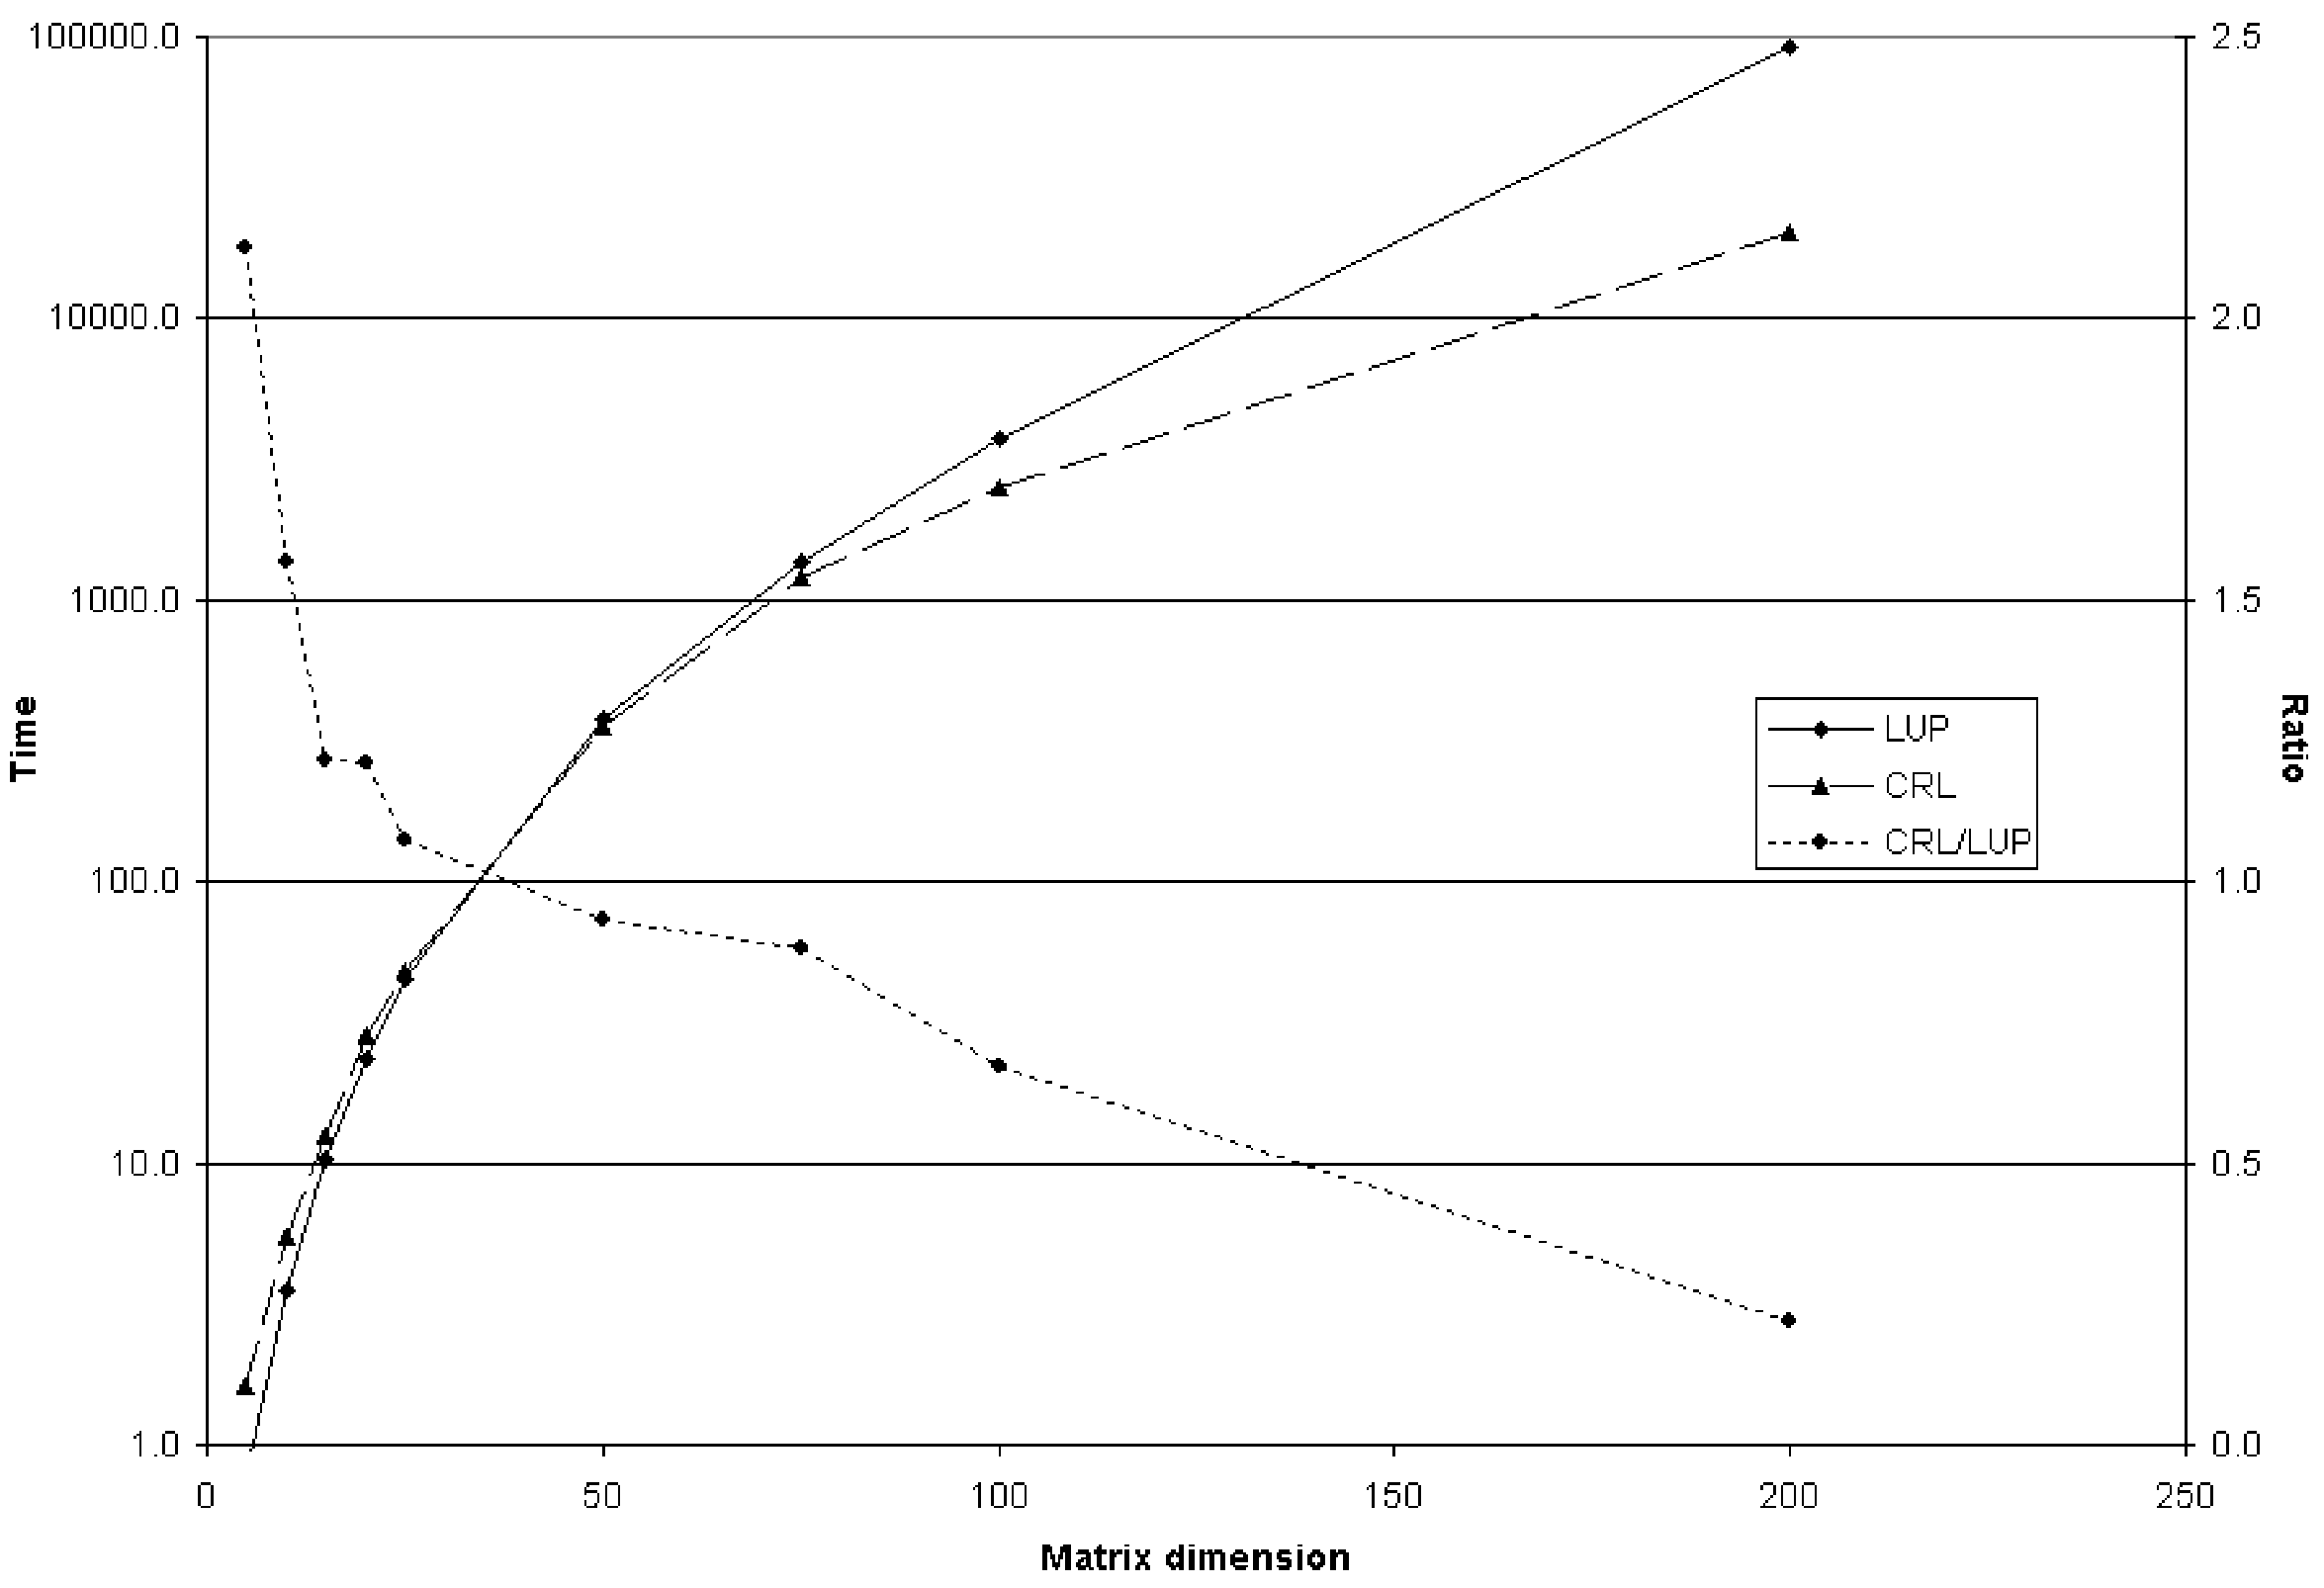
\includegraphics[width=10cm]{Figures/InversionTime}
\caption{Comparison of inversion time for non-symmetrical
matrices}\label{fig:inversionTime}
\end{figure}
Figure \ref{fig:inversionTime} shows the time needed to inverse a
non-symmetrical matrix using CRL algorithm (solid line) and LUP
decomposition (broken line), as well as the ratio between the two
times (dotted line). The CRL algorithm has a large overhead but a
smaller factor for the dependency on dimension. Thus, computing
the inverse of a matrix using LUP decomposition is faster than the
CLR algorithm for small matrices and slower for large matrices. As
a consequence, our implementation of matrix inversion uses a
different algorithm depending on the dimension of the matrix: if
the dimension of the matrix is below a critical dimension, LUP
decomposition is used; otherwise the CRL algorithm is used. In
addition, LUP decomposition is always used if it has already been
computed for another purpose.

On figure \ref{fig:inversionTime} we can determine that the
critical dimension, below which the LUP decomposition works faster
than the CRL algorithm, is about 36. These data were collected on
a Pentium II running Windows NT 4.0. As this value is depending on
the performance of the operating system, the reader is advised to
determine the critical dimension again when installing the classes
on another system.

In practice, the CLR algorithm described in equations
\ref{eq:crlsplit} to \ref{eq:crlshur} can only be applied to
symmetric matrices. In \cite{CorLeiRiv} Cormen {\it et al.}
propose to generalize it to matrices of any size by observing the
following identity:
\begin{equation}
\label{eq:pseudoinverse}
  {\bf A}\cdot\left[\left(\transpose{A}\cdot{\bf A}\right)^{-1}\cdot\transpose{A}\right]={\bf I}
\end{equation}
which can be verified for any matrix ${\bf A}$. Thus, the
expression in bracket can be considered as the inverse of the
matrix ${\bf A}$. In mathematics, it is called the pseudo-inverse
or the Moore-Penrose inverse. Since the product
$\transpose{A}\cdot{\bf A}$ is always a symmetric matrix, its
inverse can be computed with the CRL algorithm. In practice,
however. this technique is plagued with rounding errors and should
be used with caution (\cf section \ref{sec:matrixrounding}).

\subsection{Matrix inversion implementation}
Listing \ref{ls:inversion} shows the complete implementation in
Pharo. It contains additional methods for the classes {\tt
DhbMatrix} and {\tt DhbSymmetricMatrix}.

For symmetric matrices the method {\tt inverse} first tests
whether the dimension of the matrix is below a given threshold ---
defined by the class method {\tt lupCRLCriticalDimension} --- or
whether the LUP decomposition of the matrix was already performed.
In that case, the inverse is computed from the LUP decomposition
using the method described at the beginning of section
\ref{sec:matrixinversion}. Otherwise the CRL algorithm is used.
The implementation of the CRL algorithm is straightforward thanks
to the matrix operators defined in section
\ref{sec:slinearalgebra}.

For non-symmetric matrices the method {\tt inverse} first tests
whether the matrix is square or not. If the matrix is square, LUP
decomposition is used. If the matrix is not square the pseudo
inverse is computed using equation \ref{eq:pseudoinverse}.

In both cases there is no error handling. Inverting a singular
matrix produces an arithmetic error which must be handled by the
calling method.

\begin{listing}  Implementation of matrix inversion \label{ls:inversion}
$$\halign{ #\hfil&\quad#\hfil\cr {\sl Class}& {\Large\bf DhbSymmetricMatrix}\cr
{\sl Subclass of }&{\tt DhbMatrix}\cr\noalign{\vskip 1ex}
}$$


Class methods
{\parskip 1ex\par\noindent}
{\bf join:} {\tt anArrayOfMatrices}
\begin{verbatim}
    | rows n |
    rows := OrderedCollection new.
    n := 0.
    ( anArrayOfMatrices at: 1) rowsDo:
        [ :each |
          n := n + 1.
          rows add: each, ((anArrayOfMatrices at: 3) columnAt: n) ].
    n := 0.
    ( anArrayOfMatrices at: 2) rowsDo:
        [ :each |
          n := n + 1.
          rows add: ((anArrayOfMatrices at: 3) rowAt: n), each ].
    ^ self rows: rows 
\end{verbatim}
{\bf lupCRLCriticalDimension}
\begin{verbatim}
    ^ 36
\end{verbatim}



Instance methods
{\parskip 1ex\par\noindent}
{\bf crlInverse}
\begin{verbatim}
    | matrices b1 cb1ct cb1 |
    matrices := self split.
    b1 := (matrices at: 1) inverse.
    cb1 := (matrices at: 3) * b1.
    cb1ct := (cb1 productWithTransposeMatrix: (matrices at: 3)) 
                asSymmetricMatrix.
    matrices at: 3 put: (matrices at: 2) * cb1.
    matrices at: 2 put: ((matrices at: 2) accumulateNegated: cb1ct) 
                                                              inverse.
    matrices at: 1 put: ( b1 accumulate: (cb1 
                       transposeProductWithMatrix: (matrices at: 3))).
    (matrices at: 3) negate.
    ^ self class join: matrices
\end{verbatim}
{\bf inverse}
\begin{verbatim}
    ^ (rows size < self class lupCRLCriticalDimension or: 
                                           [ lupDecomposition notNil ]) 
            ifTrue: [ self lupInverse ]
            ifFalse: [ self crlInverse ]
\end{verbatim}
{\bf split}
\begin{verbatim}
    | n b d c |
    n := self largestPowerOf2SmallerThan: rows size.
    ^Array with: (self class rows: ((1 to: n) asVector collect: [ 
                               :k | (rows at: k) copyFrom: 1 to: n]))
              with:(self class rows: (((n+1) to: rows size) 
      asVector collect: [ :k | (rows at: k) copyFrom: (n+1) to: rows 
      size]))
              with: (self class superclass rows: (((n+1) to: rows 
     size) asVector collect: [ :k | (rows at: k) copyFrom: 1 to: n]))
\end{verbatim}


$$\halign{ #\hfil&\quad#\hfil\cr {\sl Class}& {\Large\bf DhbMatrix}\cr
{\sl Subclass of }&{\tt Object}\cr\noalign{\vskip 1ex}

{\sl Instance variable names:}&\parbox[t]{4 in}{\tt  rows lupDecomposition }\cr\noalign{\vskip 1ex}}$$


Class methods
{\parskip 1ex\par\noindent}
{\bf lupCRLCriticalDimension}
\begin{verbatim}
    ^ 40
\end{verbatim}

Instance methods
{\parskip 1ex\par\noindent}
{\bf inverse}
\begin{verbatim}
    ^self isSquare 
        ifTrue: [ self lupInverse ]
        ifFalse: [ self squared inverse * self transpose ]
\end{verbatim}
{\bf largestPowerOf2SmallerThan:} {\tt anInteger}
\begin{verbatim}
    | m m2|
    m := 2.
    [ m2 := m * 2.
      m2 < anInteger ] whileTrue:[ m := m2 ].
    ^ m
\end{verbatim}
{\bf lupInverse}
\begin{verbatim}
    ^ self class rows: self lupDecomposition inverseMatrixComponents
\end{verbatim}


\end{listing}


\subsection{Matrix inversion --- Rounding problems}
\label{sec:matrixrounding} Operations with large matrices are well
known to exhibit serious rounding problems. The reason is that the
computation of the vector product of each row and column is a sum:
the higher the dimension and the longer the sum. For large matrix
dimensions the magnitude of the sum can mask small contributions
from single products. Successive multiplications thus amplify
initial small deviations. This is especially the case when
computing the inverse of a general matrix using the CRL algorithm
combined with the pseudo-inverse (\ref{eq:pseudoinverse}).

Now is the time to unveil the mystery example of section
\ref{sec:roundingintro} about rounding errors propagation. The
problem solved in this example is matrix inversion. The parameter
describing the complexity of the problem is the dimension of the
matrix. This is the quantity plotted along the $x$-axis of figure
\ref{fig:precision}. Let ${\bf A}$ the matrix to be inverted. The
matrix ${\bf M}$ defined by
\begin{equation}
  {\bf M}=\inverse{A}\cdot{\bf A}-{\bf I},
\end{equation}
should have all its components equal to zero. The precision of the
result is defined as the largest absolute value over all
components of the matrix ${\bf M}$. That quantity is plotted along
the $y$-axis of figure \ref{fig:precision}.

Method A computes the inverse of the matrix using LUP
decomposition, method B using the CRL algorithm. The {\sl general}
data correspond to a matrix whose components were generated by a
random number generator (\cf section \ref{sec:random}). They were
all comprised between 0 and 1. For the {\sl special} data the
matrix ${\bf A}$ is a covariance matrix (\cf section
\ref{sec:covmatrix}) obtained by generating 1000 vectors with
random components comprised between 0 and 1. For method B general
data, the inverse of a non-symmetrical matrix is computed using
the CRL algorithm combined with equation \ref{eq:pseudoinverse}.
In this general form, the CRL algorithm is faster the LUP for
matrices of dimensions larger than about 165. The precision,
however, is totally unreliable as can been seen on Figure
\ref{fig:precision}.

\section{Matrix eigenvalues and eigenvectors of a non-symmetric matrix}
\label{sec:eigen} A non-zero vector ${\bf u}$ is called an {\sl
eigenvector} of the matrix ${\bf M}$ if there exists a complex
number $\lambda$ such that:
\begin{equation}
\label{eq:eigendef}
 {\bf M}\cdot{\bf u}=\lambda{\bf u}.
\end{equation}
the number $\lambda$ is called an {\sl eigenvalue} of the matrix
${\bf M}$. Equation \ref{eq:eigendef} implies that the matrix
${\bf M}$ must be a square matrix. In general a non-singular
matrix of dimension $n$ has $n$ eigenvalues and eigenvectors. Some
eigenvalues, however, may be double\footnote{Eigenvalues are the
roots of a polynomial of degree $n$. A double eigenvalue has two
different eigenvectors.}. Discussing the existence of eigenvalues
in the general case goes beyond the scope of this book. Equation
\ref{eq:eigendef} shows that an eigenvector is defined up to a
constant\footnote{If the vector ${\bf u}$ is an eigenvector of the
matrix ${\bf M}$ with eigenvalue $\lambda$, so are all vectors
$\alpha{\bf u}$ for any $\alpha\ne 0$.}. One can prove that two
eigenvectors of the same matrix, but corresponding to two
different eigenvalues, are orthogonal to each other \cite{Bass}.
Thus, the eigenvectors of a matrix form a complete set of
reference in a $n$ dimensional space.

Computing the eigenvalues and eigenvectors of an arbitrary matrix
is a difficult task. Solving this problem in the general case is
quite demanding numerically. In the rest of this section we give
an algorithm which works well when the absolute value of one of
the eigenvalues is much larger than that of the others. The next
section discusses Jacobi's algorithm finding all eigenvalues of a
symmetrical matrix.

For an arbitrary square matrix the eigenvalue with the largest
absolute value can be found with an iterative process. Let ${\bf
u}$ be an arbitrary vector and let $\lambda_{\max}$ be the
eigenvalue with the largest absolute value. Let us define the
following series of vectors:
\begin{mainEquation}
\left\{
  \begin{array}{lcl}
    {\bf u}_0 &=& {\bf u}, \\*[1ex]
    {\bf u}_k &=& {\displaystyle 1\over\displaystyle\lambda_{\max}}{\bf M}\cdot{\bf
    u}_{k-1}\mbox{\quad for $k>0$}.
  \end{array}
\right.
\end{mainEquation}
It is easy to prove\footnote{Hint: one must write the vector ${\bf
u}$ as a linear combination of the eigenvectors of the matrix
${\bf M}$. Such linear combination exists because the eigenvectors
of a matrix form a complete system of reference.} that:
\begin{equation}
  \lim_{k\to\infty}{\bf u}_k={\bf u}_{\max},
\end{equation}
where ${\bf u}_{\max}$ is the eigenvector corresponding to
$\lambda_{\max}$. Using this property, the following algorithm can
be applied.
\begin{enumerate}
  \item Set ${\bf u}=\left(1,1,\ldots,1\right)$.
  \item Set ${\bf u}^{\prime}={\bf M}{\bf u}$.
  \item Set $\lambda=u^{\prime}_1$, that is the first component of the
  vector ${\bf u}^{\prime}$.
  \item Set ${\bf u}= {1\over\lambda}{\bf u}^{\prime}$.
  \item Check for convergence of $\lambda$. Go to step 2 if
  convergence is not yet attained.
\end{enumerate}
The algorithm will converge toward $\lambda_{\max}$ if the initial
vector ${\bf u}$ is not an eigenvector corresponding to a null
eigenvalue of the matrix ${\bf M}$. If that is the case, one can
chose another initial vector.

Once the eigenvalue with the largest absolute value has been
found, the remaining eigenvalues can be found by replacing the
matrix ${\bf M}$ with the matrix:
\begin{equation}
\label{eq:eigennext}
  {\bf M}^{\prime}={\bf M}\cdot\left({\bf I}-{\bf u}_{\max}\otimes{\bf
  v}_{\max}\right),
\end{equation}
where ${\bf I}$ is the identity matrix of same dimension as the
matrix ${\bf M}$ and ${\bf v}_{\max}$ is the eigenvector of the
matrix $\transpose{M}$ corresponding to
$\lambda_{\max}$\footnote{The transpose of a matrix has the same
eigenvalues, but not necessarily the same eigenvectors.}. Using
the fact that eigenvectors are orthogonal to each other, one can
prove that the matrix ${\bf M}^{\prime}$ of equation
\ref{eq:eigennext} has the same eigenvalues as the matrix except
for $\lambda_{\max}$ which is replaced by 0. A complete proof of
the above can be found in \cite{Bass}.

All eigenvalues and eigenvectors of the matrix ${\bf M}$ can be
found by repeating the process above $n$ times. However, this
works well only if the absolute values of the eigenvalues differ
from each consecutive ones by at least an order of magnitude.
Otherwise, the convergence of the algorithm is not very good. In
practice, this algorithm can only be used to find the first couple
of eigenvalues.

\subsection{Finding the largest eigenvalue --- General
implementation}\marginpar{Figure \ref{fig:linearalgebraclasses}
with the box {\bf LargestEigenValueFinder} grayed.} The object in
charge of finding the largest eigenvalue is of course an instance
of a subclass of the iterative process class described in
\ref{sec:iteration}. As the reader can see very few methods are
required because most of the work is already implemented in the
framework for iterative processes. The implementation is identical
in both languages and will be discussed here. The largest
eigenvalue finder has the following instance variables:
\begin{description}
  \item[\tt matrix] the matrix whose largest eigenvalue is sought,
  \item[\tt eigenValue] the sought eigenvalue,
  \item[\tt eigenVector] the sought eigenvector and
  \item[\tt transposedEigenVector] the eigenvector of the
  transposed matrix.
\end{description}
The creation method takes the matrix as argument. Two accessor
methods are supplied to retrieve the results, the eigenvalue and
the eigenvector.

The method {\tt initializeIterations} creates a vector to the
matrix dimension and sets all its components equal to 1. As the
algorithm progresses this vector will contain the eigenvector of
the matrix. Similarly, a vector, which will contain the
eigenvector of the transposed matrix, is created in the same way.
In principle one should add a part to verify that this vector does
not correspond to a null eigenvalue of the matrix. This small
improvement is left as an exercise to the reader.

The algorithm is implemented within the single method {\tt
evaluateIteration} as described in section \ref{sec:iteration}.
The relative precision of the sought eigenvalue is the precision
used to break out of the iterative process.

Since the algorithm determines both the eigenvalue and the
eigenvector the object in charge of the algorithm keeps both of
them and must give access to both of them. Two accessor methods
are supplied to retrieve the results, the eigenvalue and the
eigenvector.

The largest eigenvalue finder is responsible to create the object
responsible for finding the next eigenvalue when needed. Thus, the
eigenvector of the transposed matrix is also computed along with
the regular eigenvector. The method {\tt
nextLargestEigenValueFinder} returns a new instance of the class,
which can be used to compute the next largest eigenvalue, by
computing a new matrix as described in equation
\ref{eq:eigennext}.

\subsection{Finding the largest eigenvalue  implementation} Listing \ref{ls:eigenlarge} shows the Pharo
implementation of the  class {\tt DhbLargestEigenValueFinder},
subclass of the class {\tt DhbIterativeProcess}.

The following code example shows how to use the class to find the
first two largest eigenvalues of a matrix.
\begin{codeExample}
\begin{verbatim}

 | m finder eigenvalue eigenvector nextFinder nextEigenvalue nextEigenvector |
 m := DhbMatrix rows: #((84 -79 58 55)
                        (-79 84 -55 -58)
                        (58 -55 84 79)
                        (55 -58 79 84)).
 finder := DhbLargestEigenValueFinder matrix: m.
 eigenvalue := finder evaluate.
 eigenvector := finder eigenvector.
 nextFinder := finder nextLargestEigenValueFinder.
 nextEigenvalue := nextFinder evaluate.
 nextEigenvector := nextFinder eigenvector.
\end{verbatim}
\end{codeExample}
First the matrix {\tt m} is defined from its components. Then, an
instance of the class {\tt DhbLargestEigenValueFinder} is created
for this matrix. The iterative process is started as described in
section \ref{sec:siteration}. Its result is the eigenvalue. The
eigenvector is retrieved using an accessor method. Then, a new
instance of {\tt DhbLargestEigenValueFinder} is obtained from the
first one. The next largest eigenvalue and its eigenvector are
retrieved from this new instance exactly as before.

\begin{listing} Implementation of the search for the largest eigenvalue
\label{ls:eigenlarge}
$$\halign{ #\hfil&\quad#\hfil\cr {\sl Class}& {\Large\bf DhbLargestEigenValueFinder}\cr
{\sl Subclass of }&{\tt DhbIterativeProcess}\cr\noalign{\vskip 1ex}

{\sl Instance variable names:}&\parbox[t]{4 in}{\tt  matrix eigenvector transposeEigenvector }\cr\noalign{\vskip 1ex}}$$


Class methods
{\parskip 1ex\par\noindent}
{\bf defaultMaximumIterations}
\begin{verbatim}
    ^ 100
\end{verbatim}
{\bf matrix:} {\tt aMatrix}
\begin{verbatim}
    ^ self new initialize: aMatrix; yourself
\end{verbatim}
{\bf matrix:} {\tt aMatrix} {\bf precision:} {\tt aNumber}
\begin{verbatim}
    ^ self new initialize: aMatrix; desiredPrecision: aNumber; 
                                                              yourself
\end{verbatim}



Instance methods
{\parskip 1ex\par\noindent}
{\bf eigenvalue}
\begin{verbatim}
    ^ result
\end{verbatim}
{\bf eigenvector}
\begin{verbatim}
    ^ eigenvector * (1 / eigenvector norm)
\end{verbatim}
{\bf evaluateIteration}
\begin{verbatim}
    | oldEigenvalue |
    oldEigenvalue := result.
    transposeEigenvector := transposeEigenvector * matrix.
    transposeEigenvector := transposeEigenvector 
                * (1 / (transposeEigenvector at: 1)).
    eigenvector := matrix * eigenvector.
    result := eigenvector at: 1.
    eigenvector := eigenvector * (1 / result).
    ^oldEigenvalue isNil 
        ifTrue: [ 2 * desiredPrecision]
        ifFalse: [ (result - oldEigenvalue) abs ]
\end{verbatim}
{\bf initialize:} {\tt aMatrix}
\begin{verbatim}
    matrix := aMatrix.
\end{verbatim}
{\bf initializeIterations}
\begin{verbatim}
    eigenvector := DhbVector new: matrix numberOfRows.
    eigenvector atAllPut: 1.0.
    transposeEigenvector := DhbVector new: eigenvector size.
    transposeEigenvector atAllPut: 1.0
\end{verbatim}
{\bf nextLargestEigenValueFinder}
\begin{verbatim}
    | norm |
    norm := 1 / (eigenvector * transposeEigenvector).
    ^self class 
        new: matrix * ((DhbSymmetricMatrix identity: eigenvector 
                                                                size) 
                        - (eigenvector * norm tensorProduct: 
                                                transposeEigenvector))
        precision: desiredPrecision
\end{verbatim}


\end{listing}


\section{Matrix eigenvalues and eigenvectors of a symmetric matrix}
\label{sec:eigensym}
In the nineteen century Carl Jacobi discovered an efficient
algorithm to find the eigenvalues of a symmetric matrix. Finding
the eigenvalues of a symmetric matrix is easier since all
eigenvalues are real.

In the section \ref{sec:eigen} we have mentioned that the
eigenvectors of a matrix are orthogonal. Let ${\bf u}^{\left( 1
\right)},\ldots,{\bf u}^{\left( n \right)}$ the set of
eigenvectors of the matrix ${\bf M}$ such that ${\bf
u}^{\left(i\right)}\cdot{\bf u}^{\left(i\right)}=1$ for all $i$.
Then, the matrix
\begin{equation}
  {\bf O}=\pmatrix{u^{\left(1\right)}_1& u^{\left(2\right)}_1&\ldots& u^{\left(n\right)}_1\cr
  u^{\left(1\right)}_2& u^{\left(2\right)}_2&\ldots& u^{\left(n\right)}_2\cr
  \vdots&\vdots&\ddots&\vdots\cr
  u^{\left(1\right)}_n& u^{\left(2\right)}_n&\ldots&
  u^{\left(n\right)}_n\cr},
\end{equation}
where $u^{\left(k\right)}_i$ is the $i^{\mathop{\rm th}}$
component of the $k^{\mathop{\rm th}}$ eigenvector,is an
orthogonal\footnote{An orthogonal matrix of dimension $n$ is a
rotation in the $n$-dimensional space.} matrix. That is, we have:
\begin{equation}
\label{eq:orthomatrix} \transpose{O}\cdot{\bf O}={\bf I}.
\end{equation}
Equation \ref{eq:orthomatrix} is just another way of stating that
the vectors ${\bf u}^{\left( 1 \right)},\ldots,{\bf u}^{\left( n
\right)}$ are orthogonal to each other and are all normalized to
1. Combining this property with the definition of an eigenvector
(equation \ref{eq:eigendef}) yields:
\begin{equation}
\transpose{O}\cdot{\bf M}\cdot{\bf O}=\pmatrix{\lambda_1&
0&\ldots&0\cr
  0& \lambda_2&\ldots& 0\cr
  \vdots&\vdots&\ddots&\vdots\cr
  0& 0&\ldots&\lambda_n\cr},
\end{equation}
where $\lambda_1,\ldots,\lambda_n$ are the eigenvalues of the
matrix ${\bf M}$.

The gist of Jacobi's algorithm is to apply a series of orthogonal
transformations such that the resulting matrix is a diagonal
matrix. It uses the fact that, for any orthogonal matrix ${\bf
R}$, the matrix $\transpose{R}{\bf M}\cdot{\bf R}$ has the same
eigenvalues as the matrix ${\bf M}$. This follows from the
definition of an eigenvector (equation \ref{eq:eigendef}) and the
property of an orthogonal matrix (equation \ref{eq:orthomatrix}).

An orthogonal matrix corresponds to a rotation of the system of
reference axes. Each step of Jacobi's algorithm is to find an
rotation, which annihilates one of the off-diagonal elements of
the matrix resulting from that orthogonal transformation. Let
${\bf R}_1$ be such matrix and let us define
\begin{equation}
  {\bf M}_1 = \transpose{R}_1\cdot{\bf M}\cdot{\bf R}_1.
\end{equation}
Now, let us define the orthogonal transformation ${\bf R}_2$,
which annihilates one of the off-diagonal elements of the matrix
${\bf M}_1$. The hope is that, after a certain number of steps
$m$, the matrix
\begin{equation}
  \begin{array}{lcl}
    {\bf M}_m & = &\transpose{R}_m\cdot{\bf M}_{m-1}\cdot{\bf
    R}_m\\*[2ex]
      & = &\transpose{R}_m\cdots\transpose{R}_1\cdot{\bf M}\cdot{\bf
      R}_1\cdots{\bf R}_m
  \end{array}
\end{equation}
becomes a diagonal matrix. Then the diagonal elements of the
matrix ${\bf M}_m$ are the eigenvalues and the matrix
\begin{equation}
    {\bf O}_m = {\bf R}_1\cdots{\bf R}_m
\end{equation}
is the matrix containing the eigenvectors.

Instead of annihilating just any diagonal element, one tries to
annihiliate the element with the largest absolute value. This
ensures the fastest possible convergence of the algorithm. Let
$m_{kl}$ be the off-diagonal element of the matrix ${\bf M}$ with
the largest absolute value. We define a matrix ${\bf R}_1$ with
components:
\begin{equation}
  \left\{
  \begin{array}{lcl}
    r^{\left(1\right)}_{kk} &=& \cos\vartheta, \\*[2ex]
    r^{\left(1\right)}_{ll} &=& \cos\vartheta, \\*[2ex]
    r^{\left(1\right)}_{kl} &=& -\sin\vartheta, \\*[2ex]
    r^{\left(1\right)}_{lk} &=& \sin\vartheta, \\*[2ex]
    r^{\left(1\right)}_{ii} &=& 1\mbox{\quad for $i\ne k,l$}, \\*[2ex]
    r^{\left(1\right)}_{ij} &=& 0\mbox{\quad for $i\ne j, i$ and $j \ne k,l$.}
  \end{array}
  \right.
\end{equation}
The reader can verify that the matrix ${\bf R}_1$ is an orthogonal
matrix. The new matrix ${\bf M}_1=\transpose{R}_1\cdot{\bf
M}\cdot{\bf R}_1$ has the same components as the matrix ${\bf M}$
except for the rows and columns $k$ and $l$. That is, we have
\begin{equation}
\label{eq:jacobistep}
  \left\{
  \begin{array}{lcl}
    m^{\left(1\right)}_{kk} &=& \cos^2\vartheta m_{kk}+\sin^2\vartheta m_{ll} - 2\sin\vartheta\cos\vartheta m_{kl}, \\*[2ex]
    m^{\left(1\right)}_{ll} &=& \sin^2\vartheta m_{kk}+\cos^2\vartheta m_{ll} + 2\sin\vartheta\cos\vartheta m_{kl}, \\*[2ex]
    m^{\left(1\right)}_{kl} &=& \left(\cos^2\vartheta-\sin^2\vartheta\right)m_{kl}+\sin\vartheta\cos\vartheta
    \left(m_{kk}-m_{ll}\right), \\*[2ex]
    m^{\left(1\right)}_{ik} &=& \cos\vartheta m_{ik}-\sin\vartheta m_{il}\mbox{\quad for $i\ne k,l$}, \\*[2ex]
    m^{\left(1\right)}_{il} &=& \cos\vartheta m_{il}+\sin\vartheta m_{ik}\mbox{\quad for $i\ne k,l$}, \\*[2ex]
    m^{\left(1\right)}_{ij} &=& m_{ij}\mbox{\quad for $i\ne k,l$ and $j\ne k,l$}.  \end{array}
  \right.
\end{equation}
In particular, the angle of rotation can be selected such that
$m^{\left(1\right)}_{kl}=0$. That condition yields the following
equation for the angle of the rotation:
\begin{equation}
\label{eq:jacobirot}
  {\cos^2\vartheta-\sin^2\vartheta
  \over\sin\vartheta\cos\vartheta}={m_{ll} - m_{kk}\over
  m_{kl}}=\alpha,
\end{equation}
where the constant $\alpha$ is defined by equation
\ref{eq:jacobirot}. Introducing the variable $t=\tan\vartheta$,
equation \ref{eq:jacobirot} can be rewritten as:
\begin{equation}
\label{eq:jacobi2nd}
  t^2+2\alpha t - 1 =0.
\end{equation}
Since equation \ref{eq:jacobi2nd} is a second order equation,
there are two solutions. To minimize rounding errors, it is
preferable to select the solution corresponding to the smallest
rotation\cite{Press}. The solution of equation \ref{eq:jacobi2nd}
has already been discussed in section \ref{sec:outsmart} for the
case where $\alpha$ is positive. For any $\alpha$, it can be
written as:
\begin{equation}
\label{eq:jacobisolinverse}
  t={\displaystyle\sign\left(\alpha\right)\over\displaystyle\left|\alpha\right|+\sqrt{\alpha^2+1}}.
\end{equation}
In fact, the value of the angle $\vartheta$ does not need to be
determined. We have:
\begin{equation}
  \left\{
  \begin{array}{lcl}
    \cos\vartheta&=&{\displaystyle 1\over\displaystyle
    \sqrt{t^2+1}},\\*[2ex]
    \sin\vartheta&=&t\cos\vartheta. \end{array}
  \right.
\end{equation}
Let us now introduce the quantities $\sigma$ and $\tau$ defined as
\begin{equation}
  \left\{
  \begin{array}{lcl}
    \sigma&=&\sin\vartheta,\\*[2ex]
    \tau&=&{\displaystyle\sin\vartheta \over\displaystyle 1+\cos\vartheta}.\end{array}
  \right.
\end{equation}
Then equations \ref{eq:jacobistep} can be rewritten as
\begin{mainEquation}
\label{eq:jacobistepfinal}
  \left\{
  \begin{array}{lcl}
    m^{\left(1\right)}_{kk} &=& m_{kk} - t m_{kl}, \\*[2ex]
    m^{\left(1\right)}_{ll} &=& m_{ll} + t m_{kl}, \\*[2ex]
    m^{\left(1\right)}_{kl} &=& 0, \\*[2ex]
    m^{\left(1\right)}_{ik} &=& m_{ik}-\sigma\left( m_{il}+\tau m_{ik}\right)\mbox{\quad for $i\ne k,l$}, \\*[2ex]
    m^{\left(1\right)}_{il} &=& m_{il}+\sigma\left( m_{ik}-\tau m_{il}\right)\mbox{\quad for $i\ne k,l$}, \\*[2ex]
    m^{\left(1\right)}_{ij} &=& m_{ij}\mbox{\quad for $i\ne k,l$ and $j\ne k,l$}.  \end{array}
  \right.
\end{mainEquation}

Finally, we must prove that the transformation above did not
increase the absolute values of the remaining off-diagonal
elements of the matrix ${\bf M}_1$. Using equations
\ref{eq:jacobistep} the sum of the off-diagonal elements of the
matrix ${\bf M}_1$ is:
\begin{equation}
\label{eq:jacobiconv}
  \sum_{i\ne j}\left(m^{\left(1\right)}_{ij}\right)^2=\sum_{i\ne j}m_{ij}^2-2 m^2_{kl}.
\end{equation}
Thus, this sum is always less that the sum of the squared
off-diagonal elements of the matrix ${\bf M}$. In other words the
algorithm will always converge.

\rubrique{Jacobi's algorithm} Now we have all the elements to
implement Jacobi's algorithm. The steps are described hereafter:
\begin{enumerate}
  \item Set the matrix ${\bf M}$ to the matrix whose eigenvalues
  are sought.
  \item Set the matrix ${\bf O}$ to an identity matrix of the same
  dimension as the matrix ${\bf M}$.
  \item Find the largest off-diagonal element, $m_{kl}$, of the matrix ${\bf
  M}$.
  \item Build the orthogonal transformation ${\bf R}_1$
  annihilating the element $m_{kl}$.
  \item Build the matrix ${\bf M}_1=\transpose{R}_1\cdot{\bf M}\cdot{\bf
  R}_1$.
  \item If $\left|m_{kl}\right|$ is less than the desired
  precision go to step 8.
  \item Let ${\bf M}={\bf M}_1$ and ${\bf O}={\bf O}\cdot{\bf R}_1$; go to step 3.
  \item The eigenvalues are the diagonal elements of the matrix ${\bf
  M}$ and the eigenvectors are the rows of the matrix ${\bf O}$.
\end{enumerate}
Strictly speaking, Jacobi's algorithm should be stopped if the
largest off-diagonal element of matrix ${\bf M}_1$ is less than
the desired precision. However, equation \ref{eq:jacobiconv}
guaranties that the largest off-diagonal element of the matrix
after each step of Jacobi's algorithm is always smaller that the
largest off-diagonal element of the matrix before the step. Thus.
the stopping criteria proposed above can safely be used. This
slight overkill prevents us from scanning the off-diagonal
elements twice per step.

As the algorithm converges, $\alpha$ becomes very large. As
discussed in section \ref{sec:outsmart}, the solution of equation
\ref{eq:jacobi2nd} can be approximated with
\begin{equation}
  t\approx{\displaystyle 1\over\displaystyle 2\alpha}.
\end{equation}
This expression is used when the computation of $\alpha^2$ causes
an overflow while evaluating equation \ref{eq:jacobisolinverse}.

\subsection{Jacobi's algorithm --- General implementation}
\marginpar{Figure \ref{fig:linearalgebraclasses} with the box {\bf
JacobiTransformation} grayed.}Jacobi's algorithm is an iterative
algorithm. The object implementing Jacobi's algorithm is a
instance of the class {\tt JacobiTransform}; it is a subclass of
the iterative process discussed in section \ref{sec:iteration}.
The instance variables of this class are different in the two
language implementations.

When an instance of the class {\tt JacobiTransform} is created,
the matrix whose eigenvalues are sought is copied into the matrix
${\bf M}$. This permits to use the same storage over the duration
of the algorithm since equations \ref{eq:jacobistepfinal} can be
evaluated in place. Actually, only the upper half of the
components needs to be stored since the matrix is a symmetric
matrix.

The method {\tt evaluateIteration} finds the largest off-diagonal
element and performs the Jacobi step (equations
\ref{eq:jacobistepfinal}) for that element. During the search for
the largest off-diagonal element, the precision of the iterative
process is set to the absolute value of the largest off-diagonal
element. This is one example where it does not make sense to
compute a relative precision. Actually, the precision returned by
the method {\tt evaluateIteration} is that of the previous
iteration, but it does not really matter to make one iteration too
much.

The method {\tt finalizeIterations} performs a bubble sort to
place the eigenvalues in decreasing order of absolute value.
Bubble sorting is used instead of using a {\tt SortedCollection}
because one must also exchange the corresponding eigenvectors.

The result of the iterative process is an array containing the
sorted eigenvalues plus the transformation matrix ${\bf O}$
containing the eigenvectors. Extracting these results is language
dependent.

\subsection{Jacobi's algorithm implementation}
Listing \ref{ls:jacobi} shows the implementation of
Jacobi's algorithm.

The following code example shows how to use the class to find the
eigenvalues and eigenvectors of a symmetric matrix.
\begin{codeExample}
\begin{verbatim}

 | m jacobi eigenvalues eigenvectors |
 m := DhbSymmetricMatrix rows: #((84 -79 58 55)
                                 (-79 84 -55 -58)
                                 (58 -55 84 79)
                                 (55 -58 79 84)).
 jacobi := DhbJacobiTransformation matrix: m.
 eigenvalues := jacobi evaluate.
 eigenvectors := jacobi transform columnsCollect: [ :each | each].
\end{verbatim}
\end{codeExample}
First the matrix {\tt m} is defined from its components. Then, an
instance of the class {\tt DhbJacobiTransformation} is created for
this matrix. The iterative process is started as described in
section \ref{sec:siteration}. Its result is an array containing
the eigenvalues sorted in decreasing order. The corresponding
eigenvectors are retrieved from the columns of the matrix ${\bf
O}$ obtained from the method {\tt transform}.

The class {\tt DhbJacobiTransformation} has two instance variables
\begin{description}
  \item[\tt lowerRows] an array of array containing the lower part
  of the matrix and
  \item[\tt transform] the components of the matrix ${\bf O}$.
\end{description}
Since the matrix ${\bf M}$ is symmetric there is no need to keep
all of its components. This not only reduces storage but also
speeds up somewhat the algorithm because one only need to
transform the lower part of the matrix.


The instance variable {\tt result} contains the sorted eigenvalues
at the end of the iterative process. The method {\tt transform}
returns the symmetric matrix ${\bf O}$ whose columns contain the
eigenvectors in the same order. The code example shown at the
beginning of this section shows how to obtain the eigenvectors
from the matrix.

\begin{listing} Implementation of Jacobi's algorithm \label{ls:jacobi}
$$\halign{ #\hfil&\quad#\hfil\cr {\sl Class}& {\Large\bf DhbJacobiTransformation}\cr
{\sl Subclass of }&{\tt DhbIterativeProcess}\cr\noalign{\vskip 1ex}

{\sl Instance variable names:}&\parbox[t]{4 in}{\tt  lowerRows transform }\cr\noalign{\vskip 1ex}}$$


Class methods
{\parskip 1ex\par\noindent}
{\bf matrix:} {\tt aSymmetricMatrix}
\begin{verbatim}
    ^ super new initialize: aSymmetricMatrix
\end{verbatim}
{\bf new}
\begin{verbatim}
    ^ self error: 'Illegal creation message for this class'
\end{verbatim}

Instance methods
{\parskip 1ex\par\noindent}
{\bf evaluateIteration}
\begin{verbatim}
    | indices |
    indices := self largestOffDiagonalIndices.
    self transformAt: (indices at: 1) and: (indices at: 2).
    ^ precision

\end{verbatim}
{\bf exchangeAt:} {\tt anInteger}
\begin{verbatim}
    | temp n |
    n := anInteger + 1.
    temp := result at: n.
    result at: n put: ( result at: anInteger).
    result at: anInteger put: temp.
    transform do:
        [ :each |
          temp := each at: n.
          each at: n put: ( each at: anInteger).
          each at: anInteger put: temp ].
\end{verbatim}
{\bf finalizeIterations}
\begin{verbatim}
    | n |
    n := 0.
    result := lowerRows collect: 
                    [ :each | 
                    n := n + 1.
                    each at: n ].
    self sortEigenValues
\end{verbatim}
{\bf initialize:} {\tt aSymmetricMatrix}
\begin{verbatim}
    | n m |
    n := aSymmetricMatrix numberOfRows.
    lowerRows := Array new: n.
    transform := Array new: n.
    1 to: n do:
        [ :k |
          lowerRows at: k put: ( ( aSymmetricMatrix rowAt: k) 
                                                   copyFrom: 1 to: k).
          transform at: k put: ( ( Array new: n) atAllPut: 0; at: k 
                                                    put: 1; yourself) ].
    ^ self
\end{verbatim}
{\bf largestOffDiagonalIndices}
\begin{verbatim}
    | n m abs |
    n := 2.
    m := 1.
    precision := ( ( lowerRows at: n) at: m) abs.
    1 to: lowerRows size do:
        [ :i |
          1 to: ( i - 1) do:
            [ :j |
              abs := ( ( lowerRows at: i) at: j) abs.
              abs > precision
                ifTrue: [ n := i.
                          m := j.
                          precision := abs ] ] ].
    ^ Array with: m with: n
\end{verbatim}
{\bf printOn:} {\tt aStream}
\begin{verbatim}
    | first |
    first := true.
    lowerRows do: 
        [ :each |
          first ifTrue: [ first := false ]
                 ifFalse: [ aStream cr ].
          each printOn: aStream ].
\end{verbatim}
{\bf sortEigenValues}
\begin{verbatim}
    | n bound m |
    n := lowerRows size.
    bound := n.
    [ bound = 0 ]
        whileFalse: [ m := 0.
                      1 to: bound - 1 do:
                        [ :j |
                          (result at: j) abs > (result at: j + 1) abs
                            ifFalse: [ self exchangeAt: j.
                                      m := j ] ].
                        bound := m ].
\end{verbatim}
{\bf transform}
\begin{verbatim}
    ^ DhbMatrix rows: transform
\end{verbatim}
{\bf transformAt:} {\tt anInteger1} {\bf and:} {\tt anInteger2}
\begin{verbatim}
    | d t s c tau apq app aqq arp arq |
    apq := ( lowerRows at: anInteger2) at: anInteger1.
    apq = 0
        ifTrue: [ ^ nil ].
    app := (lowerRows at: anInteger1) at: anInteger1.
    aqq := (lowerRows at: anInteger2) at: anInteger2.
    d := aqq - app.
    arp := d * 0.5 / apq.
    t := arp > 0 
        ifTrue: [ 1 / ( ( arp squared + 1) sqrt + arp)]
        ifFalse:[ 1 / ( arp - ( arp squared + 1) sqrt)].
    c := 1 / ( t squared + 1) sqrt.
    s := t * c.
    tau := s / ( 1 + c).
    1 to: (anInteger1 - 1)
        do: [ :r |
              arp := (lowerRows at: anInteger1) at: r.
              arq := (lowerRows at: anInteger2) at: r.
              (lowerRows at: anInteger1) at: r put: ( arp - ( s * 
                                                  (tau * arp + arq))).
              (lowerRows at: anInteger2) at: r put: ( arq + ( s * 
                                                (arp - (tau * arq)))).
            ].
    ( anInteger1 + 1) to: ( anInteger2 - 1)
        do: [ :r |
              arp := (lowerRows at: r) at: anInteger1.
              arq := (lowerRows at: anInteger2) at: r.
              (lowerRows at: r) at: anInteger1 put: ( arp - ( s * 
                                                  (tau * arp + arq))).
              (lowerRows at: anInteger2) at: r put: ( arq + ( s * 
                                                (arp - (tau * arq)))).
            ].
    ( anInteger2 + 1) to: lowerRows size
        do: [ :r |
              arp := ( lowerRows at: r) at: anInteger1.
              arq := ( lowerRows at: r) at: anInteger2.
              (lowerRows at: r) at: anInteger1 put: ( arp - ( s * 
                                                  (tau * arp + arq))).
              (lowerRows at: r) at: anInteger2 put: ( arq + ( s * 
                                                (arp - (tau * arq)))).
            ].
    1 to: lowerRows size
        do: [ :r |
              arp := ( transform at: r) at: anInteger1.
              arq := ( transform at: r) at: anInteger2.
              (transform at: r) at: anInteger1 put: ( arp - ( s * 
                                                  (tau * arp + arq))).
              (transform at: r) at: anInteger2 put: ( arq + ( s * 
                                                (arp - (tau * arq)))).
            ].
    (lowerRows at: anInteger1) at: anInteger1 put: ( app - (t * 
                                                                apq)).
    (lowerRows at: anInteger2) at: anInteger2 put: ( aqq + (t * 
                                                                apq)).
    (lowerRows at: anInteger2) at: anInteger1 put: 0.
\end{verbatim}


\end{listing}

\ifx\wholebook\relax\else\end{document}\fi
